% mnras_template.tex
%
% LaTeX template for creating an MNRAS paper
%
% v3.0 released 14 May 2015
% (version numbers match those of mnras.cls)
%
% Copyright (C) Royal Astronomical Society 2015
% Authors:
% Keith T. Smith (Royal Astronomical Society)

% Change log
%
% v3.0 May 2015
%    Renamed to match the new package name
%    Version number matches mnras.cls
%    A few minor tweaks to wording
% v1.0 September 2013
%    Beta testing only - never publicly released
%    First version: a simple (ish) template for creating an MNRAS paper

%%%%%%%%%%%%%%%%%%%%%%%%%%%%%%%%%%%%%%%%%%%%%%%%%%
% Basic setup. Most papers should leave these options alone.
\documentclass[usenatbib]{mnras}
%\pdfminorversion=5

% MNRAS is set in Times font. If you don't have this installed (most LaTeX
% installations will be fine) or prefer the old Computer Modern fonts, comment
% out the following line
%\usepackage{newtxtext,newtxmath}
% Depending on your LaTeX fonts installation, you might get better results with one of these:
%\usepackage{mathptmx}
%\usepackage{txfonts}

% Use vector fonts, so it zooms properly in on-screen viewing software
% Don't change these lines unless you know what you are doing
\usepackage[T1]{fontenc}
\usepackage{ae,aecompl}
\usepackage{hyperref}
%\usepackage{ulem}

%%%%% AUTHORS - PLACE YOUR OWN PACKAGES HERE %%%%%

% Only include extra packages if you really need them. Common packages are:
\usepackage{graphicx}	% Including figure files
\usepackage{amsmath}	% Advanced maths commands
\usepackage{amssymb}	% Extra maths symbols
\usepackage{multirow}
\usepackage[usenames,dvipsnames,svgnames,table]{xcolor}
\usepackage{verbatim}

%\hypersetup{draft}

%%%%%%%%%%%%%%%%%%%%%%%%%%%%%%%%%%%%%%%%%%%%%%%%%%

%%%%% AUTHORS - PLACE YOUR OWN COMMANDS HERE %%%%%

% Please keep new commands to a minimum, and use \newcommand not \def to avoid
% overwriting existing commands. Example:
%\newcommand{\pcm}{\,cm$^{-2}$}	% per cm-squared

\newcommand{\homsun}{\,h^{-1} {\rm M_\odot}}
\newcommand{\hmsun}{\,h^{-2} {\rm M_\odot}}
\newcommand{\msun}{{\rm M_\odot}}
\newcommand{\hkpc}{\, h^{-1}{\rm{kpc}} }
\newcommand{\hMpc}{\, h^{-1}{\rm{Mpc}} }
\newcommand{\magn}{\, {\rm mag} }
\newcommand{\mpss}{\, {\rm m}\,{\rm s}^{-2} }

\newcommand{\lan}{\langle}
\newcommand{\ran}{\rangle}

\newcommand{\lcdm}{{\rm \Lambda CDM}}
\newcommand{\am}{\, {\rm arcmin}}
\newcommand{\as}{\, {\rm arcsec}}
\newcommand*{\meanl}[1]{\overline{#1}}
\newcommand*{\meanb}[1]{\langle{#1}\rangle}
\newcommand*{\E}[1]{\times 10^{#1}}
\newcommand{\un}[1]{_{\rm #1}}
\newcommand{\dex}{\, {\rm dex}}

\newcommand*{\swap}[2]{#2#1}

%%%%%%%%%%%%%%%%%%%%%%%%%%%%%%%%%%%%%%%%%%%%%%%%%%

%%%%%%%%%%%%%%%%%%% TITLE PAGE %%%%%%%%%%%%%%%%%%%

% Title of the paper, and the short title which is used in the headers.
% Keep the title short and informative.
\title[Extending the RAR using weak lensing with KiDS-1000]{Extending the radial acceleration relation using weak gravitational lensing with KiDS-1000}
% The list of authors, and the short list which is used in the headers.
% If you need two or more lines of authors, add an extra line using \newauthor
\author[M. M. Brouwer et al.]{Margot M. Brouwer$^{1,2}$\thanks{E-mail:brouwer@astro.rug.nl}, Kyle A. Oman$^{1,3}$, Edwin A. Valentijn$^{1}$, et al.
	 %Group 1:
	 %Group 2:
	 %Group 3:
	\\
	\\
	% List of institutions
	$^{1}$Kapteyn Astronomical Institute, University of Groningen, PO Box 800, NL-9700 AV Groningen, the Netherlands.\\
	$^{2}$Institute for Theoretical Physics, University of Amsterdam, Science Park 904, 1098 XH Amsterdam, The Netherlands. \\
    $^{3}$Institute for Computational Cosmology, Department of Physics, Durham University, South Road, Durham DH1 3LE, UK \\
}

% These dates will be filled out by the publisher
\date{Accepted XXX. Received YYY; in original form ZZZ}

% Enter the current year, for the copyright statements etc.
\pubyear{2019}

% Don't change these lines
\begin{document}
\label{firstpage}
\pagerange{\pageref{firstpage}--\pageref{lastpage}}
\maketitle

% Abstract of the paper
% 266 words
\begin{abstract}
  The radial acceleration relation (RAR) measures the correlation between the gravitational acceleration expected from baryonic matter ($g\un{bar}$) and the one observed ($g\un{obs}$), traditionally using galaxy rotation curves. We use the $1006 \deg^2$ Kilo-Degree Survey (KiDS-1000) weak gravitational lensing data to extend the RAR of isolated galaxies by $2$ decades in $g_{\rm obs}$ compared to previous measurements (up to $g\un{obs}=10^{-12.5}\mpss$), finding an approximately $g\un{obs}\propto\sqrt{g\un{bar}}$ scaling across the entire range measured. We compare our measurements to the predictions of two modified gravity (MG) models: Modified Newtonian Dynamics (MOND) and Verlinde's Emergent Gravity (EG), and find that both can describe our measurements within the statistical and systematic uncertainties. We also compare with two $\lcdm$ numerical simulations: MICE and BAHAMAS. The former surprisingly closely reproduces the KiDS RAR -- the steep outer density profiles of dark matter haloes would imply a steeper low-acceleration RAR in a naive analysis, but additional lensing by structure outside the lens galaxies flattens the mock lensing-derived MICE RAR. The latter is a poor match, but this is driven by a strong bias in the stellar masses of isolated BAHAMAS galaxies. Our large sample of $\sim318\,000$ isolated lens galaxies allows us to split it by stellar mass, colour and S\'ersic index. We find a significant difference between the lensing RAR of red and blue galaxies at fixed stellar mass, which is difficult to explain within MG models. We predict that future cosmological surveys (such as Euclid) can use the lensing RAR to distinguish between MG and $\lcdm$ models, but only if systematic uncertainties in the baryonic mass distribution around galaxies are reduced.
\end{abstract}


% Select between one and six entries from the list of approved keywords.
% Don't make up new ones.
\begin{keywords}
gravitational lensing: weak -- Surveys -- methods: statistical -- galaxies: haloes -- cosmology: dark matter, theory -- gravitation.
\\
\end{keywords}

%\newpage
\clearpage

%%%%%%%%%%%%%%%%%%%%%%%%%%%%%%%%%%%%%%%%%%%%%%%%%%

%%%%%%%%%%%%%%%%% BODY OF PAPER %%%%%%%%%%%%%%%%%%


\section{Introduction}
\label{sec:introduction}

It has been known for several decades that the outer regions of galaxies rotate faster than would be expected from Newtonian dynamics based on their luminous, or `baryonic', mass. This was first discovered by \cite{bosma1981} through measuring hydrogen profiles at radii beyond the optical discs of galaxies, and \cite{rubin1983} through measuring galactic rotation curves within the optical discs. The excess gravity implied by these measurements has generally been attributed to an unknown and invisible substance named dark matter (DM), a term coined more than forty years prior by \cite{zwicky1937} when he discovered the so-called `missing mass problem' through the dynamics of galaxies in clusters.

Following more recent observations using weak gravitational lensing \cite[WL,][]{hoekstra2004,linden2014,mandelbaum2015}, baryon acoustic oscillations \cite[BAO,][]{eisenstein2005,blake2011} and the cosmic microwave background \cite[CMB,][]{spergel2003,planck2014}, cold dark matter\footnote{DM particles that moved at non-relativistic speeds at the time of recombination, as favoured by measurements of the CMB \cite[]{planck2014} and the Lyman-$\alpha$ forest \cite[]{viel2013}.} (CDM) became a key ingredient of the current standard model of cosmology: the $\lcdm$ model. In this paradigm, CDM accounts for $\Omega\un{CDM}=0.266$ of the critical density in the Universe, while baryonic matter only accounts for $\Omega\un{bar}=0.049$ \cite[]{planck2018}. The cosmological constant $\Lambda$, which is necessary to explain the accelerated expansion of the Universe and is usually associated with Dark Energy (DE), accounts for $\Omega\un{\Lambda}=0.685$.

Although the $\lcdm$ model successfully describes the behaviour of DM on a wide range of scales, no conclusive evidence for the existence of DM particles has been found so far \cite[despite years of enormous effort; for an overview, see][]{bertone2005,bertone2018}. \textcolor{black}{Combined with other problems currently defying general relativity (GR), such as the elusive unification with quantum mechanics and the mysterious nature of DE, this leaves room for alternative theories of gravity. Two modified gravity (MG) theories that deny the existence of particle DM are} modified Newtonian dynamics \cite[MOND,][]{milgrom1983} and the more recent theory of emergent gravity \cite[EG,][]{verlinde2016}. In these theories all gravity is due to the baryonic matter (or, in the case of EG, the interaction between baryons and the entropy associated with DE). Hence, one of the main properties of these theories is that the mass discrepancy in galaxies correlates strongly with their baryonic mass distribution.

Such a correlation has indeed been observed, such as via the Tully-Fisher relation \cite[TFR,][]{tully1977} between the luminosity of a spiral galaxy and its asymptotic rotation velocity \cite[]{pierce1988,bernstein1994}. This relation was later generalized as the `baryonic' TFR \cite[BTFR,][]{mcgaugh2000,mcgaugh2012} to include non-stellar forms of baryonic matter. \textcolor{black}{Even earlier}, astronomers had found a strong correlation between the observed rotation velocity as a function of galaxy radius $v\un{obs}(r)$ and the enclosed luminous mass $M\un{bar}(<r)$ \cite[]{sanders1986,sanders1996,mcgaugh2004,sanders2007,wu2015}. Since $M\un{bar}(<r)$ corresponds to the \emph{expected} gravitational acceleration $g\un{bar}(r)$ from baryonic matter, and the observed gravitational acceleration can be calculated through $g\un{obs}(r)=v\un{obs}^2(r)/r$, this relation has also been named the radial acceleration relation (RAR)\footnote{Another closely related (though slightly different) relation is the mass-discrepency acceleration relation (MDAR), which shows the expected baryonic acceleration against the discrepancy between the baryonic and the observed mass: $M\un{obs}-M\un{bar}$ \cite[see][]{mcgaugh2004}. Although measuring the MDAR requires the same data, we prefer the RAR because it's observables ($g\un{bar}$ and $g\un{obs}$) are uncorrelated.}.

Particularly \citet[][hereafter M16]{mcgaugh2016} have measured the RAR with unprecedented accuracy, using the Spitzer Photometry and Accurate Rotation Curves \cite[SPARC,][]{lelli2016b} data of 153 late-type galaxies. Their results \textcolor{black}{again} showed a tight correlation between $g\un{obs}$ and $g\un{bar}$, which they could describe using a simple double power law (eq.~4 in M16) depending only on $g\un{bar}$ and one free parameter: the acceleration scale $g\un{\dagger}$ where Newtonian gravity appears to break down. This \textcolor{black}{rekindled} the interest of scientists working on alternative theories of gravity \cite[]{lelli2017a,lelli2017b,burrage2017,li2018,obrien2019}, but also of those in favour of an explanation of the RAR within the $\lcdm$ framework, employing correlations between the masses, sizes and DM content of galaxies \cite[]{keller2017,desmond2017,ludlow2017,tenneti2018}.

The latter possibility was quantified by \citet[][hereafter N17]{navarro2017}, who used a range of simplifying assumptions based on galaxy observations and DM simulations in order to create an analytical galaxy+halo model. The goal of their model was to reconstruct the RAR inside galaxy discs, in particular the value of $a\un{0}$: the acceleration scale where the relation transitions from the baryon-dominated to the DM-dominated regime (which is equivalent to $g\un{\dagger}$), and $a\un{min}$: the minimum acceleration probed by galaxy discs. Based on their results, they claimed that the RAR can be explained within the $\lcdm$ framework at the accelerations probed by galaxy rotation curves (within the galaxy disc, i.e. $g\un{obs}>a\un{min}$). However, since their model relies on the fact that luminous kinematic tracers in galaxies only probe a limited radial range, N17 predicted that extending observations to radii beyond the disc (which correspond to lower gravitational accelerations) would lead to systematic deviations from the simple double power law proposed by M16.

The goal of this work is to extend observations of the RAR to lower accelerations, which are not measurable using galaxy rotation curves. To this end we use gravitational lensing: the perturbation of light inside a gravitational potential as described by GR. In particular, we use the method of galaxy-galaxy lensing (GGL): the statistical measurement of the coherent image distortion (shear) of a field of background galaxies (sources) by the gravitational potential of a sample of foreground galaxies \cite[lenses; for examples, see e.g.][]{fischer2000ggl,hoekstra2004,mandelbaum2006,uitert2016}. Using GGL we can measure the average (apparent) density distribution of galaxies up to a radius of $3\,{\rm Mpc}$, roughly $100$ times larger than the radius of the luminous disc ($\sim 30\,{\rm kpc}$). At our stellar mass scale of interest -- $\log(M_\star/\hmsun) \approx 10.5$ -- this radius corresponds to $g\un{bar}\approx10^{-15} \mpss$, which is $3$ orders of magnitude lower than the accelerations measurable with galaxy rotation curves\footnote{We note that this value of $g\un{bar}$ only takes into account the stellar and cold gas mass of the galaxy. In Sect. \ref{sec:baryonic_mass} we show that the contributions of hot gas, dust and `missing baryons' could increase this value to $g\un{bar}\approx10^{-14}\mpss$, which is still $2$ orders of magnitude lower than the accelerations measurable with galaxy rotation curves.}.

First, we measure the baryonic and total density profiles of our galaxies through their luminosities and GGL profiles. These measurements will be performed using 9-band photometric data from Sloan Digital Sky Survey \cite[SDSS,]{abazajian2009} and the VISTA Kilo-Degree Infrared Galaxy Survey \cite[VIKING]{edge2013}, and $1006 \deg^2$ of WL data from the Kilo-Degree Survey \textcolor{black}{\cite[KiDS-1000;][]{dejong2013,kuijken2019}}. We then translate these measurements into the baryonic and observed radial accelerations, $g\un{bar}$ and $g\un{obs}$. Finally, we compare the resulting RAR to predictions from different modified gravity (MG) theories (MOND and EG) and $\lcdm$. To test the former, we need to make the assumption that the deflection of light by gravitational potentials (as described in GR) holds in these modified theories, which we motivate in the relevant sections. \textcolor{black}{This work can be seen as an extension of \cite{brouwer2017}, where we tested the predictions of EG using GGL with $180 \deg^2$ of KiDS-GAMA data, but now with a 5 times larger survey area.}

The $\lcdm$ predictions will not only be provided by the N17 analytical model, but also by mock galaxy catalogues based on two different DM simulations. One is the Marenostrum Institut de Ci{\`e}ncies de l'Espai (MICE) Galaxy and Halo Light-cone catalogue \cite[]{carretero2015,hoffmann2015}, which is based on the MICE Grand Challenge lightcone simulation \cite[MICE-GC,][]{fosalba2015a,fosalba2015b,crocce2015}. The other mock galaxy catalogue is based on a suite of large-volume cosmological hydrodynamical simulations, which is called the BAryons and HAloes of MAssive Systems (BAHAMAS) project \cite[]{mccarthy2017}.

Having more than 1 million foreground galaxies at our disposal allows us to select specific galaxy samples, designed to optimally test the predictions from the aforementioned MG and $\lcdm$ models. Particularly, we note that the analytical models (MOND, EG and N17) mostly focus on the description of individual, isolated galaxies. In order to test them, we select a sample of galaxies whose GGL profiles are minimally affected by neighbouring galaxies (satellites) within the radius of our measurement. In contrast, the predictions from simulations can be tested with both isolated and non-isolated galaxy samples.

\textcolor{black}{The main goal of our work is to find how the RAR of isolated galaxies continues at lower accelerations (beyond the observable galaxy disc), and to distinguish which of the aforementioned MG and $\lcdm$ models best describe this result. In addition, our sample of $\sim318,000$ isolated lens galaxies allows us to split them based on observables such as stellar mass, colour and S\'ersic index. Because MG and $\lcdm$ give different predictions regarding the dependence of the RAR on these observables, this allows us to better distinguish between the different models. Specifically: according to the MOND and EG theories the relation between $g\un{bar}$ and $g\un{obs}$ should remain fixed in the regime beyond the baryon-dominated galaxy disc, and hence independent of galaxy observables. Within the $\lcdm$ paradigm, the relation between $g\un{bar}$ and $g\un{obs}$ is based on the stellar-to-halo-mass relation (SHMR) that is not necessarily constant as a function of galaxy stellar mass (or even other observables such as morphological type).}

Our paper is structured as follows: In Sect.~\ref{sec:data} we introduce our main datasets: both the \textcolor{black}{KiDS-1000} and GAMA galaxy surveys which are used to perform the GGL measurements, and the MICE and BAHAMAS simulations \& mock galaxy catalogues to which we compare our results. Sect.~\ref{sec:analysis} describes our analysis of these datasets as we select our isolated lens galaxy sample and perform the GGL measurements, \textcolor{black}{and Sect.~\ref{sec:conversion} describes how we translate these results into the RAR.} Sect.~\ref{sec:theories} contains a description of the theoretical predictions to which we compare our observations: MOND, EG and the N17 analytical DM model. \textcolor{black}{In the two sections that follow we present our resulting RAR measurements and compare them to the different models, respectively using all isolated galaxies (Sect.~\ref{sec:results}) and splitting them by different observables (Sect.~\ref{sec:results-observables}).} Sect.~\ref{sec:discon} contains the discussion and conclusion.

Throughout this work we adopt the WMAP 9-year \cite[]{hinshaw2013} cosmological parameters: $\Omega\un{m}=0.2793$, $\Omega\un{b}=0.0463$, $\Omega\un{\Lambda}=0.7207$, $\sigma_8=0.821$ and $H_0 = 70 \, {\rm km \, s^{-1} Mpc^{-1}}$, which were used as the basis of the BAHAMAS simulation. Only when dealing with the MICE simulations we use the cosmological parameters used in creating MICE, which are: $\Omega\un{m}=0.25$, $\sigma_8=0.8$, $\Omega\un{\Lambda}=0.75$, and $H_0 = 70 \, {\rm km \, s^{-1} Mpc^{-1}}$. Throughout the paper we use the reduced Hubble constant $h \equiv h_{70} = \ H_0 / (70 \, {\rm km \, s^{-1} Mpc^{-1}})$.

\section{Data}
\label{sec:data}

\subsection{KiDS source galaxies}
\label{sec:kids}

We use GGL to measure the gravitational potential around a sample of foreground galaxies (lenses), by measuring the image distortion (shear) of a field of background galaxies (sources). These sources are observed using OmegaCAM \cite[]{kuijken2011}: a 268-million pixel CCD mosaic camera mounted on the VLT Survey Telescope \cite[]{capaccioli2011}. Over the past seven years these instruments have performed KiDS, a photometric survey in the $ugri$ bands, which is especially designed to perform WL measurements \cite[]{dejong2013}.

GGL studies with KiDS have hitherto been performed in combination with the spectroscopic GAMA survey (see Sect.~\ref{sec:gama} below). Already since the previous data release \cite[KiDS-DR3,][]{dejong2017} the KiDS survey completely covers the $286 \deg^2$ GAMA area. Although the final survey will span $1350 \deg^2$ on the sky, the current state-of-the-art is the $4^{\rm th}$ Data Release \cite[KiDS-DR4,][]{kuijken2019} containing observations from $1006$ square-degree survey tiles. The measurement of the source shapes and photometric redshifts are performed in similar fashion to \cite{dejong2017}. Changes and improvements to these methods are described in \cite{kuijken2019}. 

The measurements of the galaxy shapes are based on the $r$-band data, since this filter was used during the darkest time (moon distance $> 90 \deg$) and with the best atmospheric seeing conditions ($<0.8 \as$). The $r$-band observations are co-added using the {\scshape Theli} pipeline \cite[]{erben2013}, which is improved through the addition of an illumination correction. From these images the galaxy positions are detected through the {\scshape SExtractor} algorithm \cite[]{bertin1996}. After detection, the shapes of the galaxies are measured using the \emph{lens}fit pipeline \cite[]{miller2007,miller2013}, which includes a self-calibration algorithm based on \cite{fenechconti2017}. Each shape is accompanied by a \emph{lens}fit weight $w\un{s}$, which gives an estimate of the precision of the ellipticity measurement.

For the purpose of creating the photometric redshift and stellar mass estimates, 9 bands are observed in total. The $ugri$ bands are observed by KiDS, while the VIKING survey \cite[]{edge2013} performed on the VISTA telescope adds the $ZYJHK\un{s}$ bands. All bands are reduced and co-added using the Astro-WISE pipeline \cite[AW,][]{mcfarland2013}. The galaxy colours, which form the basis of the photometric redshift measurements, are measured from these images using the Gaussian Aperture and PSF pipeline \cite[GAaP,][]{kuijken2008,kuijken2015}.

The addition of the lower frequency VISTA data allows us to extend the redshift estimates out to $0.1<z\un{B}<1.2$ (instead of $0.1<z\un{B}<0.9$ in KiDS-DR3), where $z\un{B}$ is the best-fit photometric redshift of the sources \cite[]{benitez2000,hildebrandt2012}. However, when performing our lensing measurements (see Sect.~\ref{sec:lensing}) we use the total redshift probability distribution function (PDF) $n\un{z}$ of the full source population. This $n\un{z}$ is calculated using the direct calibration method \cite[DIR,][]{hildebrandt2017}, and circumvents the inherent bias related to photometric redshift estimates of individual sources.

\subsection{GAMA foreground galaxies}
\label{sec:gama}

Although the most contraining RAR measurements will be performed using exclusively KiDS-DR4 data, the smaller set of foreground galaxies observed by the spectroscopic GAMA survey \cite[]{driver2011} functions both as a model and validation sample for the KiDS foreground galaxies. The survey was performed by the Anglo-Australian Telescope with the AAOmega spectrograph, and targeted more than $180 \, 000$ galaxies that were selected from SDSS. For this study we use the GAMA II data release \cite[]{liske2015} consisting of three equatorial regions (G09, G12 and G15). These regions span a total area of $\sim180 \deg^2$ on the sky, completely overlapping with KiDS.

GAMA has a redshift range of $0<z<0.5$, with a mean redshift of $\meanb{z}=0.22$. The survey has a redshift completeness of $98.5$~per~cent down to Petrosian $r$-band magnitude $m\un{r,Petro} = 19.8 \magn$. We limit our GAMA foreground sample to galaxies with the recommended redshift quality: $n\un{Q}\geq3$. Despite being a smaller survey, GAMA's accurate spectroscopic redshifts are highly advantageous when measuring the ESD profiles of galaxies (see Sect.~\ref{sec:lensing}). The GAMA redshifts are used to train the photometric machine-learning (ML) redshifts of our larger sample of KiDS foreground galaxies (see Sect.~\ref{sec:gamalike_kids}). Also, in combination with its high redshift completeness, GAMA allows for a more accurate selection of isolated galaxies. We therefore check that the results from the KiDS-only measurements are consistent with those from KiDS-GAMA.

To measure the RAR with KiDS-GAMA, we need individual stellar masses $M_\star$ for each GAMA galaxy. These are computed from their $ugrizZYJHK$ Spectral Energy Distributions (SEDs)\footnote{The SEDs are constrained to the rest frame wavelenght range $3000-110000$ \AA.} measured by SDSS and VIKING, by fitting them with \cite{bruzual2003} Stellar Population Synthesis (SPS) models using the Initial Mass Function (IMF) of \cite{chabrier2003}. Following the procedure described by \cite{taylor2011}, we account for flux falling outside the automatically selected aperture using the `flux-scale' correction.

\subsection{KiDS foreground selection}
\label{sec:gamalike_kids}

As our lenses, we select a `GAMA-like' (GL) sample of foreground galaxies from $1006 \deg^2$ of KiDS-DR4 data \cite[KiDS-1000,][]{kuijken2019}. To mimic the magnitude limit of GAMA ($m\un{r,Petro}<19.8 \magn$), we apply a similar cut to the (much deeper) KiDS survey. Because the KiDS catalogue does not contain Petrosian magnitudes, we use the calibrated Kron-like elliptical aperture $r$-band magnitudes `MAG\_AUTO\_CALIB' from \textsc{SExtractor}, which have a very similar distribution. Through matching the KiDS and GAMA galaxies and seeking the best trade-off between completeness and purity, we decide to limit our GL-KIDS sample to $m\un{r,auto}<20.0$. In addition, we limit the redshifts of the GL-KiDS galaxies to the maximum GAMA redshift ($z<0.5$).

\textcolor{black}{To remove stars from our galaxy sample} we apply three independent cuts, based respectively on galaxy morphology, the 9-band photometry, and the SExtractor star/galaxy classifier\footnote{Our star-galaxy separation corresponds to applying the following flags: SG2DPHOT=0, SG\_FLAG=1, CLASS\_STAR<0.5.}. We also remove galaxies that are affected by readout and diffraction spikes, saturation cores, bad pixels, or by primary, secondary or tertiary haloes of bright stars\footnote{This masking corresponds to applying all MASK values (1, 2, 4, 8, 16, 32 and 64) described in App. A.1.1 of \cite{kuijken2019}, through applying the flag: IMAFLAGS\_ISO=0.}. In addition, we apply the recommended `9-band no AW-$r$-band mask', which is also used to create the KiDS-DR4 shear catalogues\footnote{This masking corresponds to the 9-band MASK bit values 2 to 11, 13 and 14, described in App. A.2 of \cite{kuijken2019}. For more information on these masks, we refer the reader to App. A of \cite{kuijken2019}.}. Our final sample of GL-KiDS lenses consists of $1.23\E{6}$ galaxies, \textcolor{black}{almost a factor 7 more than the GAMA galaxies. This increased lens sample allows us to verify the results from \cite{brouwer2017} with increased statistics, and to study possible dependencies of the RAR on galaxy observables.}

To use the GL-KiDS sample as lenses to measure $g\un{obs}$, we need accurate individual redshifts for all galaxies in our sample. These photometric redshifts $z\un{ANN}$ are derived from the full 9-band KiDS+VIKING photometry (see Sect.~\ref{sec:kids}), by training on the spectroscopic GAMA redshifts (see Sect.~\ref{sec:gama}) using the ANNz2 (Artificial Neural Network) machine learning method \cite[]{sadeh2016,dejong2017,bilicki2017}. Objects that are not detected in all 9 bands are removed from the sample. When comparing this $z\un{ANN}$ to the spectroscopic GAMA redshifts $z\un{G}$ measured for the same galaxies, we find that their mean offset $\meanb{(z\un{ANN} - z\un{G})/(1+z\un{G})} = 9.29\E{-4}$. However, this offset is mainly caused by the low-redshift galaxies: $z\un{ANN}<0.1$. Removing these decreases the mean offset to $\meanb{\delta z/(1+z\un{G})} = -5.86\E{-5}$, with a standard deviation $\sigma\un{z} = \sigma(\delta z) = 0.026$. This corresponds to a redshift-dependent deviation of $\sigma\un{z}/(1+\meanb{z\un{ANN}})=0.02$ based on the mean redshift $\meanb{z\un{ANN}} = 0.25$ of GL-KiDS between $0.1<z<0.5$, which is the lens redshift range we use throughout this work for all lens samples.

In order to measure the expected baryonic acceleration $g\un{bar}$, we compute GL-KiDS stellar masses $M_\star$ based on these ANNz2 redshifts and the 9-band GAaP photometry. Because the GAaP photometry only measures the galaxy magnitude within a specific aperture size, the stellar mass is corrected using the `fluxscale' parameter\footnote{This fluxscale correction is applied as follows: $M_\star$ = M\_BEST + (MAG\_GAAP\_r - MAG\_AUTO\_CALIB) / 2.5.}. The stellar masses are computed by the \textsc{LePhare} algorithm \cite[]{arnouts1999, ilbert2006}, which performs SPS model fits on the stellar component of the galaxy SED. The used SPS model is \cite{bruzual2003}, with the IMF from \citet[][equal to those used for the GAMA stellar masses]{chabrier2003}. \textsc{LePhare} provides both the best-fit value `MASS\_BEST' of the galaxy template PDF, and the $68$~per~cent confidence level upper and lower limits. We can use the latter to estimate the statistical uncertainty on $M_\star$. For both the upper and lower limit, the mean difference with the best-fit mass is approximately: $|\log_{10}\lan M\un{lim}/M\un{best} \ran| \approx 0.06 \dex$.

Another way of estimating the statistical uncertainty in the stellar mass is to combine the estimated uncertainties from the input: the redshifts and magnitudes. The redshift uncertainty $\sigma\un{z}/\meanb{z\un{G}} = 0.11$ corresponds to an uncertainty in the luminosity distance of: $\sigma(\delta D\un{L})/\meanb{D\un{L}} = 0.12$. We take the flux $F$ to remain constant between measurements, such that: $4 \pi D\un{L}^2 F \propto D\un{L}^2 \propto L$. Assuming that approximately $L \propto M_\star$ we can estimate: 
\begin{equation}
\frac{M_\star + \delta M_\star}{M_\star} = \frac{D\un{L}(\meanl{z}) + D\un{L}(\meanl{z}+\delta z)^2}{D\un{L}(\meanl{z})^2} \, ,
\end{equation}
which finally gives us our stellar mass uncertainty resulting from the GL-KiDS redshifts: $\log_{10}(1+\delta M_\star/M_\star) = 0.11 \dex$. The uncertainty resulting from the GL-KiDS magnitudes is best estimated by comparing two different KiDS apparent magnitude measurements: the elliptical aperture magnitudes `MAG\_AUTO\_CALIB' from \textsc{SExtractor} and the S\'ersic magnitudes `MAG\_AUTO\_2dphot' from \textsc{2DPHOT}. The standard deviation of their difference is $\sigma(\delta m) = 0.14$, which corresponds to a flux ratio of $1.14$ (or $0.057 \dex$). Using the same assumption, now taking $D\un{L}$ to remain constant, results in: $4 \pi D\un{L}^2 F \propto F \propto L \propto M_\star$. This means our flux ratio directly corresponds to our estimate of the $M_\star$ uncertainty. Quadratically combining the $0.11 \dex$ uncertainty from the redshifts and the $0.057 \dex$ uncertainty from the magnitudes gives us an estimate of the total statistical uncertainty on the stellar mass of $\sim0.12$. This is about twice the estimate from the \textsc{LePhare} code, which does not include the redshift uncertainties.

When comparing $M\un{\star,ANN}$ with the GAMA stellar masses $M\un{\star,G}$ of matched galaxies, we find that its distribution is very similar, with a standard deviation of $0.21 \dex$ around the mean. Nevertheless there exists a systematic offset of $\log(M\un{\star,ANN}) - \log(M\un{\star,G}) = -0.056 \dex$, which is caused by the different stellar mass estimation methods used on the two surveys. In general, it has been found impossible to constrain stellar masses within a systematic uncertainty of $\Delta M_\star \approx 0.2 \dex$ when applying different methods, even when the same SPS, IMF and data are used \cite[]{taylor2011,wright2017}. We therefore normalize the $M\un{\star,ANN}$ values of our GL-KiDS sample to the mean $M\un{\star,G}$ of GAMA, while indicating throughout our results the range of possible bias due to a $\Delta M_\star = 0.2 \dex$ systematic shift in $M_\star$. We estimate the effect of this bias by computing the RAR with $\log_{10}(M_\star)\pm\Delta M_\star$ as upper/lower limits.

\subsection{MICE mock galaxies}
\label{sec:mice_mocks}

In order to compare our observations to $\lcdm$-based predictions, we use two different sets of simulations. One of these is the MICE-GC $N$-body simulation, which contains $\sim 7\E{10}$ DM particles in a $(3072 \hMpc)^3$ comoving volume \cite[]{fosalba2015b}. From this simulation the MICE collaboration constructed a $\sim5000\deg^2$ lightcone with a maximum redshift of $z=1.4$. The DM halos in this lightcone are identified using a Friend-of-Friend (FOF) algorithm on the particles. These DM halos were populated with galaxies using a hybrid halo occupation distribution (HOD) and halo abundance matching (HAM) prescription \cite[]{carretero2015,crocce2015}. \textcolor{black}{The galaxy luminosity function and colour distribution of these galaxies are constructed to reproduce local observational constraints provided by the SDSS \cite[]{blanton2003a, blanton2003b, blanton2005}.}

In the MICECATv2.0 catalogue\footnote{The MICECATv2.0 catalogue is available through CosmoHub (\url{https://cosmohub.pic.es}).} which we use in this work, every galaxy has sky coordinates, redshifts, comoving distances, apparent magnitudes and absolute magnitudes assigned to them. Of the total MICE lightcone we use $1024\deg^2$, an area similar to the KiDS-1000 survey. We use the SDSS apparent $r$-band magnitudes $m\un{r}$, as these most closely match those from KiDS \cite[see][]{brouwer2018}. We can therefore limit the MICE galaxies to the same apparent magnitude as the GL-KiDS sample: $m\un{r}<20 \, {\rm mag}$, in order to create a GL-MICE foreground galaxy (lens) sample. We also use the same redshift limit: $0.1<z<0.5$, resulting in a mean GL-MICE redshift $\meanb{z}=0.23$, almost equal to that of GAMA and GL-KiDS within this range. The absolute magnitudes of the mock galaxies go down to $M\un{r} - 5\log_{10}(h) < -14 \magn$, which corresponds to the faintest GAMA and GL-KiDS galaxies. New to this version is that each galaxy is also assigned a stellar mass $M_\star$, which is needed to compute the RAR (see Sect.~\ref{sec:conversion}). These stellar masses are determined from the galaxy luminosities $L$ using \cite{bell2001} $M/L$ ratios.

In addition, each galaxy has a pair of lensing shear values associated with it ($\gamma_1$ and $\gamma_2$, with respect to the Cartesian coordinate system). These shear values were calculated from healpix weak lensing maps that were constructed using the `onion shell method' \cite[]{fosalba2008, fosalba2015a}. The lensing map of MICECATv2.0 has an improved resolution of $0.43$ arcmin, which is almost twice smaller than that of MICECATv1.0 ($0.85$ arcmin). Throughout this work, we will not use MICE results within a radius $R\un{res}$ corresponding to 3 times this resolution. We always calculate $R\un{res}$ and the corresponding $g\un{bar}$ using the mean angular diameter distance and baryonic mass of the used MICE lens sample. For the full sample of isolated MICE galaxies these values are: $R\un{res}=0.25 \hMpc$ and $g\un{bar}=6.60\E{-14} \mpss$.

At scales larger than this resolution limit, the MICE shears allow us emulate the GGL analysis and conversion to the RAR that we perform on our KiDS-1000 data (as described in Sect.~\ref{sec:analysis}) using the MICE simulation. To create a sample of MICE background galaxies (sources) for the lensing analysis, we apply limits on the MICE mock galaxies' redshifts and apparent magnitudes which are analogous to those applied to the KiDS source sample: $0.1 < z < 1.2$, $m\un{r}>20$ (see \citealp{hildebrandt2017} and Sect.~\ref{sec:kids}; note that uncertainties in the KiDS $z\un{B}$ are not accounted for in this selection). We also apply an absolute magnitude cut of $M\un{r}>-18.5 \, {\rm mag}$, in order to resemble the KiDS source redshift distribution more closely.

The MICE-GC mock catalogue also features very accurate clustering. At lower redshifts ($z<0.25$) the clustering of the mock galaxies as a function of luminosity is constructed to reproduce the SDSS clustering observations \cite[]{zehavi2011}, while at higher redshifts ($0.45<z<1.1$) it was validated against the Cosmic Evolution Survey \cite[COSMOS,][]{ilbert2009}. This makes MICE especially suitable to reproduce the RAR at larger scales ($>0.3\hMpc$) where neighbouring galaxies start to affect the lensing signal, and to test our criteria considering the galaxy isolation (see Sect.~\ref{sec:isolation}).

% From Crocce (2015): By construction our catalogue reproduces the local observational  constraints  provided  by  the  Sloan  Digital  SkySurvey (SDSS, York et al. (2000)). We reproduce the local luminosity function (Blanton et al. 2003) and color distributions (Blanton et al. 2003, 2005). The method has also been adjusted to match the clustering as a function of luminosity and color following observational constraints from the SDSS (Zehavi et al. 2011).

\subsection{BAHAMAS mock galaxies}
\label{sec:bahamas_mocks}
The second set of simulations which we utilize is the BAHAMAS (BAryons and HAloes of MAssive Systems) suite of \citet{mccarthy2017}. The BAHAMAS runs are smoothed-particle hydrodynamical realizations of $(400 \, h^{-1}\un{100} {\rm kpc})^3$ volumes and include prescriptions for radiative cooling/heating, ionizing background radiation, star formation, stellar evolution \& chemical enrichment, (kinetic wind) supernova feedback, supermassive black hole accretion, and merging \& thermal AGN feedback. The simulations are calibrated to reproduce the stellar and hot gas content of massive haloes, which makes them particularly well-suited for our study of the matter content around haloes out to distances of $1$--$3\hMpc$. The masses of DM and baryonic resolution elements are $3.85\times 10^9$ and $7.66\times 10^8 \, h^{-1}\un{100} {\rm M_\odot}$ respectively, and the gravitational softening is fixed at $\epsilon = 4 \, h^{-1}\un{100} {\rm kpc} = 5.71 \hkpc$.

Haloes and galaxies are identified in the simulations using the FOF \citep{davis1985} and Subfind \citep{springel2001a,dolag2009} algorithms. We label the most massive subhalo in each FOF group as the `central' and other subhaloes as `satellites'. We construct an `isolated' galaxy sample by restricting the selection to central subhaloes which have no other subhaloes (satellites or centrals) more massive than $10$~per~cent of their mass within $3 \hMpc$. We randomly select $100$ galaxies per $0.25$ dex bin in $M_{200}$ between $10^{12}$ and $10^{13.5} \hmsun$. In the last two bins there are less than $100$ candidates, so we select them all. All galaxies have a redshift $z=0.25$. For each selected galaxy we construct an integrated surface density map, integrated along the line-of-sight (LOS) for $\pm 15 \, {\rm comoving} \, h^{-1}\un{100} {\rm Mpc})^3$ around the target halo. We also extract the cumulative spherically averaged mass profile of each target subhalo, decomposed into DM, stars, and gas. For both the maps and profiles, we include mass contributions from all surrounding (sub)structures, i.e. we do not isolate the haloes from their surrounding environment.

We use the integrated surface density map of each galaxy to calculate its mock excess surface density profile as a function of the projected distance $R$ from the lens centre, in order to mimic the effect of GGL and the conversion to the RAR on the BAHAMAS results. Each pixel on these maps corresponds to $15 \, {\rm comoving} \,  h^{-1}\un{100} {\rm kpc}$, which in our physical units is: $15 / (1+z) \, 0.7^{-1} h^{-1}\un{70} {\rm kpc} = 17.14 \hMpc$. The density maps each have a dimensionality of $400 \times 400$ pixels. Hence the total area of each map is $(6.86 \hMpc)^2$. In calculating the ESD and RAR with BAHAMAS we follow, as closely as possible, the GGL procedure and conversion to the RAR as described in Sect.~\ref{sec:analysis}. We truncate our ESD profiles at $10$ times the gravitational softening length: $10 \, \epsilon = 0.057 \hMpc$, to avoid the numerically poorly-converged central region \cite[]{power2003}. For the full sample of isolated BAHAMAS galaxies, this corresponds to $g\un{bar}=2.38\E{-12} \mpss$.

\section{Data analysis}
\label{sec:analysis}

\subsection{Lensing measurement}
\label{sec:lensing}

The measurement of the projected mass density that we use to estimate the gravitational acceleration around galaxies (see Sect.~\ref{sec:conversion}), is obtained through the WL method \cite[for a general introduction, see][]{bartelmann2001,schneider2006}. More specifically, we use GGL: the measurement of the coherent image distortion of a field of background galaxies (sources) by the gravitational potential of a sample of foreground galaxies (lenses). Because the individual image distortions are very small (only $\sim1$~per~cent compared to the galaxy's unknown original shape), this method can only be performed statistically for a large sample of sources. We average their projected ellipticity component tangential to the direction of the lens galaxy, $\epsilon\un{t}$, which is the sum of the intrinsic ellipticity $\epsilon\un{int}$ and the tangential shear $\gamma\un{t}$ caused by WL. Assuming no preferential alignment in the intrinsic galaxy shapes ($\lan\epsilon\un{int}\ran=0$), the average $\lan\epsilon\un{t}\ran$ is an estimator for $\gamma\un{t}$. By measuring this averaged quantity in circular annuli around the lens centre, we obtain the tangential shear profile $\gamma\un{t}(R)$ as a function of projected radius $R$. Because our final goal is to compute $g\un{obs}$ as a function of $g\un{bar}$, we choose our $R$-bins such that they correspond to $15$ logarithmic bins between $1\E{-15} < g\un{bar} < 5\E{-12} \mpss$. For each individual lens the calculation of these $g\un{bar}$-bins is based on the baryonic mass of the galaxy $M\un{gal}$ (see Sect.~\ref{sec:conversion}). In real space this binning approximately corresponds to the distance range used in \cite{brouwer2017}: $0.03 < R < 3 \hMpc$.

The lensing shear profile can be related to the physical excess surface density (ESD, denoted $\Delta\Sigma$) profile:
\begin{equation}
	\Delta \Sigma (R) = \Sigma\un{crit} \gamma\un{t}(R) = \meanb{\Sigma}(<R) - \Sigma(R) \, ,
	\label{eq:deltasigma}
\end{equation}
which is the surface density $\Sigma(R)$ at projected radius $R$, subtracted from the average surface density $\meanb{\Sigma(<R)}$ within $R$. The conversion factor between $\gamma\un{t}$ and $\Delta\Sigma$ is the critical surface density, whose inverse is also called the lensing efficiency:
\begin{equation}
	\Sigma\un{crit}^{-1} = \frac{4\pi G}{c^2} \int_{0}^{\infty} D(z\un{l}) \left( \int_{z\un{l}}^{\infty}  \frac{D(z\un{l}, z\un{s})}{D(z\un{s})} n(z\un{s}) \, {\rm d} z\un{s} \right) p(z\un{l}) \, {\rm d} z\un{l} \, .
	\label{eq:sigmacrit}
\end{equation}
Here $D(z\un{l})$ and $D(z\un{s})$ are the angular diameter distances to the lens and the source respectively, and $D(z\un{l}, z\un{s})$ the distance between them. The constant multiplication factor is defined by Newton's gravitational constant $G$ and the speed of light $c$. For the lens redshifts $z\un{l}$, we use the ANNz machine-learning redshifts of the KiDS foreground galaxy sample (see Sect.~\ref{sec:gamalike_kids}). We implement the contribution of $z\un{l}$ by integrating over the individual redshift probability distributions $p(z\un{l})$ of each lens. This $p(z\un{l})$ is defined by a normal distribution centred at the lens' $z\un{ANN}$ redshift, with a standard deviation: $\sigma\un{z}/(1+z) = 0.02$ (which is equal to the standard deviation of GL-KiDS redshifts compared to their matched spectroscopic GAMA redshifts, see Sect.~\ref{sec:kids}). For the source redshifts $z\un{s}$ we follow the method used in \cite{dvornik2018}, by integrating over the part of the redshift probability distribution $n(z\un{s})$ where $z\un{s}>z\un{l}$. In addition, sources only contribute their shear to the lensing signal when $z\un{B}+\Delta z > z\un{l}$, i.e. the sum of their best-fit photometric redshift $z\un{B}$ and the redshift buffer $\Delta z=0.2$ is greater than the lens redshift.

To increase the signal-to-noise ($S/N$) ratio of the lensing signal even further, the ESD profile is averaged (or `stacked') for large samples of lenses. We define a lensing weight $W\un{ls}$ which depends on both the \emph{lens}fit weight $w\un{s}$ and the lensing efficiency $\Sigma\un{crit}^{-1}$:
\begin{equation}
	W\un{ls} = w\un{s} \left( \Sigma\un{crit,ls}^{-1} \right)^2 \, ,
	\label{eq:weights}
\end{equation}
and use it to optimally sum the measurements from all lens-source pairs into the average ESD:
\begin{equation}
	\Delta\Sigma = \frac{1}{1+\mu} \frac{\sum_{ls} W_{ls} \, \epsilon_{{\rm t},ls} \, \Sigma_{{\rm crit},ls} }{ \sum_{ls}{W_{ls}} }  \, .
	\label{eq:ESDmeasured}
\end{equation}
Here the factor (1+$\mu$) corrects for the `multiplicative bias' \cite[]{fenechconti2017}. Extending the method of \cite{dvornik2017} to the higher KiDS-DR4 redshifts, $\mu$ is calculated from the multiplicative bias corrections $m$ of the individual sources:
\begin{equation}
	\mu=\frac{\sum_{s} w_{s} m_{s}}{\sum_{ls} w_{s}} \, ,
	\label{eq:biascorr}
\end{equation}
in 11 linear redshift bins between \mbox{$0.1<z\un{B}<1.2$}. The value of this correction is $\mu\approx0.014$, independent of the projected distance from the lens. After correction, the effects of the multiplicative bias are reduced to $<1$~per~cent.

We also correct our lensing signal for effects from residual shape correlations due to the (small) PSF anisotropy of the KiDS observations. At the survey edges, it is possible that the averaging of the source shapes is not performed over all azimuthal angles, which can result in systematic effects on the ESD at larger scales ($R>1\hMpc$). We correct for this by subtracting the ESD profile measured around $\sim5$ million uniform random coordinates, $50$ times the size of our total GL-KiDS sample. These random coordinates mimic the exact footprint of KiDS, excluding the areas masked by the `9-band no AW-$r$-band' mask that we apply to the GL-KiDS lenses (see Sect.~\ref{sec:gamalike_kids}). In order to create random redshift values that mimic the true distribution, we create a histogram of the GL-KiDS redshifts divided into $80$ linear bins between $0.1<z\un{ANN}<0.5$. In each bin, we create random redshift values equal to the number of real lenses in that bin. Because of the large contiguous area of KiDS-DR4, we find that the random ESD profile is very small at all projected radii $R$, with a mean absolute value of only $\sim2$~per~cent of the lensing signal of the isolated GL-KiDS galaxies. 

The error values on the ESD profile are estimated by the square-root of the diagonal of the analytical covariance matrix, which is described in sec.~3.4 of \cite{viola2015}. The full covariance matrix is calculated based on the contribution of each individual source to the ESD profile, and incorporates the correlation between sources that contribute to the ESD in multiple bins, both in projected distance $R$ and in galaxy observable.

The GGL method described above is basically identical to the procedure used by recent KiDS-GGL papers, specifically: \cite{dvornik2017,dvornik2018} and \cite{brouwer2017,brouwer2018}. For more details on the KiDS-GGL procedure, we recommend reading these recent works. The method that was used in older works \cite[]{viola2015,sifon2015,uitert2016,brouwer2016} is also very similar, although small changes have occurred in the pipeline with the arrival of new data-releases.

Note that we use the unadulterated GGL method throughout this work, also when testing the MOND and EG theories. We recognize that, by using the basic GGL equations to measure the (apparent) density distributions in these frameworks, we necessarily assume that the laws of GR hold with respect to the deflection of light by a gravitational potential. We therefore motivate in Sect.~\ref{sec:MOND} and \ref{sec:EG} why this assumption holds for the alternative gravity theories that we test in this work.


\subsection{Isolated galaxy selection}
\label{sec:isolation}

\begin{figure}
	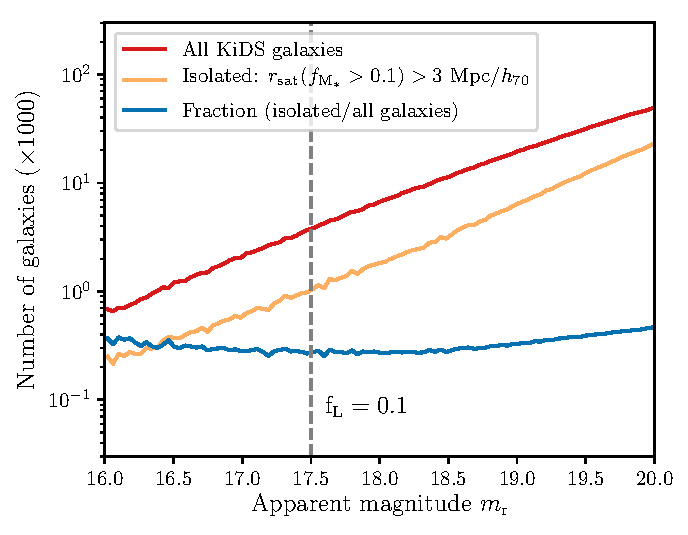
\includegraphics[width=1.0\columnwidth]{Figures/isolation_test_kids_perc0p1-3Mpc.pdf}
	\caption{The number of isolated galaxies (orange line) compared to the total number of galaxies (red line), as a function of apparent $r$-band magnitude $m\un{r}$. The dashed vertical line represents the magnitude $m\un{bright}$, below which \emph{all} satellites with a luminosity fraction larger than $f\un{L} \equiv L\un{sat}/L\un{lens}=0.1$ compared to the lens are still detected. Beyond this limit, the fraction of isolated/all galaxies (blue line) slightly increases because satellites fainter than the flux limit are not detected, which can cause lenses close to the magnitude limit ($m\un{lim}=20 \magn$) to be falsely identified as isolated.}
	\label{fig:isolation_test_fraction}
\end{figure}

\begin{figure}
	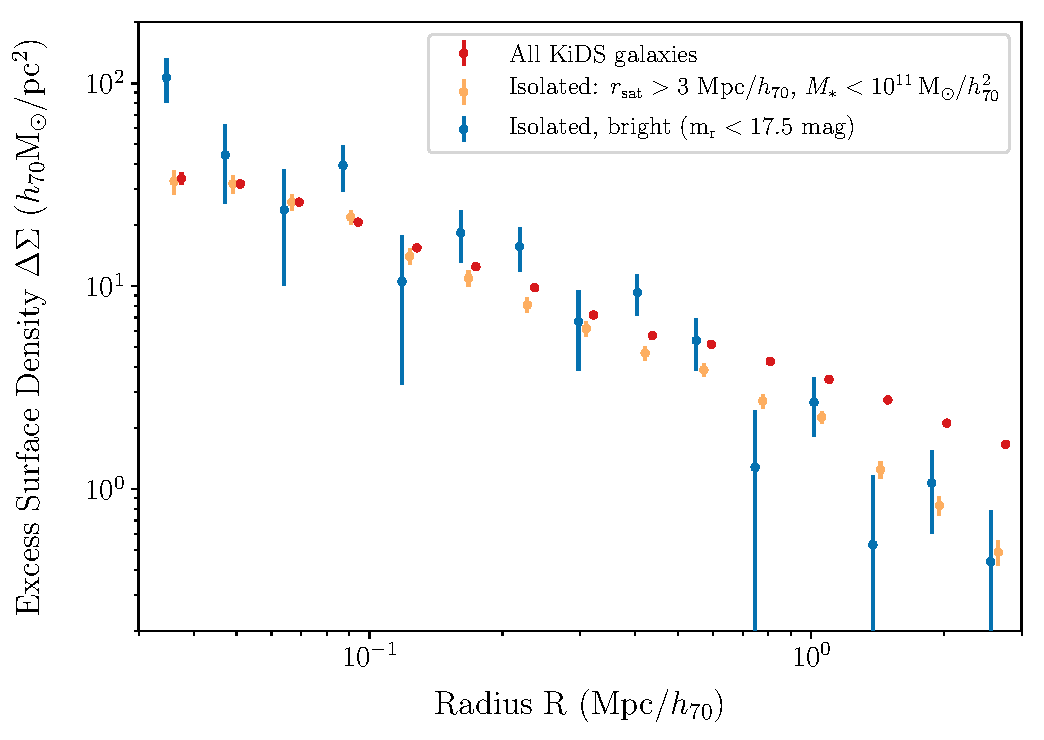
\includegraphics[width=1.0\columnwidth]{Figures/ESD_KiDS_isotest.pdf}
	\caption{To assess the effect of the \textcolor{black}{GL-KiDS} magnitude limit ($m\un{r}<20 \magn$) on the isolation criterion, we compare the ESD profiles of our full sample of isolated \textcolor{black}{GL-KiDS} galaxies (red points with $1\sigma$ error bars) with that of a more reliable `bright' sample (dark blue, $m\un{r}<17.5 \magn$) which allows us to see \emph{all} satellites down to luminosity fraction $f\un{L} \equiv L\un{sat}/L\un{lens}=0.1$. Due to the smaller number of lenses, the ESD profile of the bright isolated sample shows much larger error bars and scatter. Nevertheless, its behaviour on both small and large scales is consistent with the ESD profile of the full isolated sample, indicating that the effect of the magnitude limit is limited.}
	\label{fig:isolation_test_ESD}
\end{figure}

\begin{figure}
	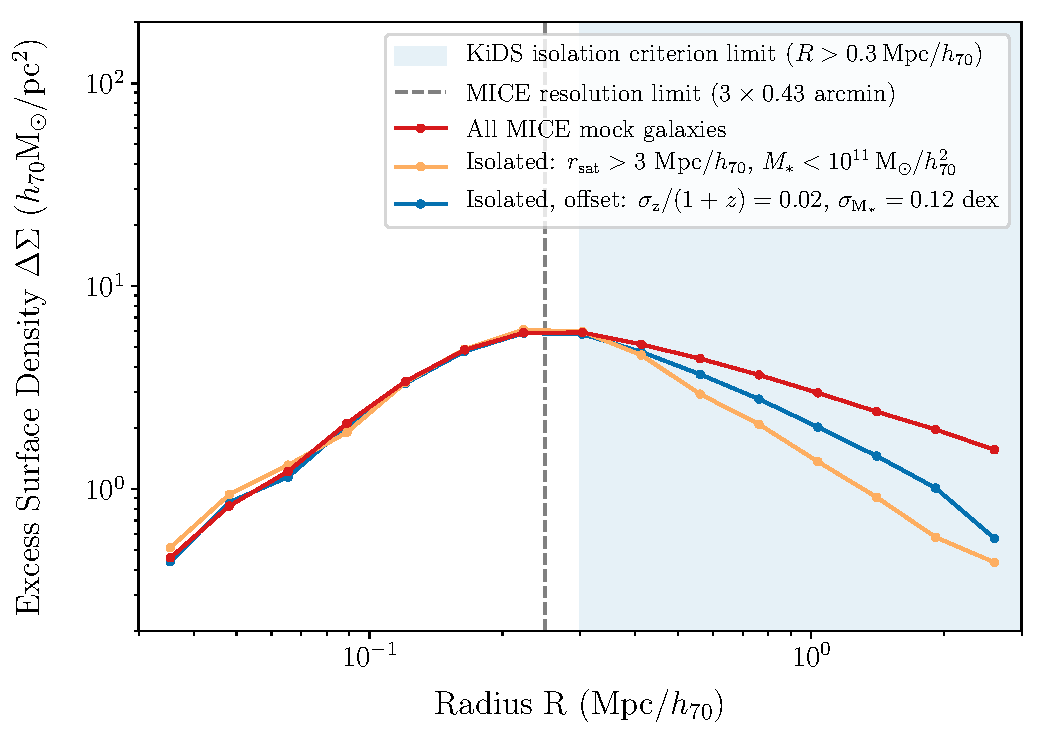
\includegraphics[width=1.0\columnwidth]{Figures/ESD_MICE_isotest_offset.pdf}
	\caption{The ESD profile of the `offset' isolated MICE sample (blue line) is created by using MICE galaxies with randomly offset redshifts ($\sigma\un{z}/(1+z) = 0.02$) and stellar masses ($\sigma\un{M_\star} = 0.12 \dex$) when selecting the isolated lenses, in order to mimic the effect of the GL-KiDS measurement uncertainties on the isolation criterion. Compared to the ESD profile of the truly isolated MICE sample (orange line) the offset sample has a $\sim30$~per~cent higher signal at large scales due to the contribution of satellites. We therefore take extra care when comparing GL-KiDS results at $R > 0.3 \hMpc$ (light blue region). Nevertheless, the ESD of the offset isolated MICE sample is significantly lower than that of all MICE galaxies (red line), created without any isolation criterion. In addition, we show the radius corresponding to 3 times the resolution of the MICE simulation (dashed line), which in the case of the isolated MICE sample is $R<0.25$. Throughout this work, we only use the MICE results beyond this radius.}
	\label{fig:isolation_test_offset}
\end{figure}

After performing the measurement of the RAR using GGL, our final goal is to compare the results to different analytical models (Sect.~\ref{sec:theories}) and N-body simulations (Sects.~\ref{sec:mice_mocks} and \ref{sec:bahamas_mocks}) which make specific predictions on the galaxy-halo connection. While the simulations are designed to describe galaxies in their cosmological environment, the analytical models mainly focus on the description of individual galaxies. This means that, in order to test these models, we need to select galaxies that are relatively isolated. Most importantly, their measured ESD profiles should not be significantly affected by neighbouring galaxies, which we call `satellites'. We define our isolated lenses such that they not have any satellites with more than a fraction $f\un{M_\star} \equiv M\un{\star,sat}/M\un{\star,lens}$ of their stellar mass within a spherical radius $r\un{sat}$. We choose $f\un{M_\star}=0.1$ which corresponds to $10$~per~cent of the lens stellar mass, and $r\un{sat}=3\hMpc$ which is equal to the maximum projected radius of our measurement. In short: $r\un{sat}(f\un{M_\star}>0.1)>3\hMpc$. We also restrict our lens stellar masses to $M_\star < 10^{11} \hmsun$, since galaxies with higher masses have significantly more satellites (see Sect.~2.2.3 of \citealp{brouwer2017}).

We validate this isolation criterion using the GL-KiDS data and -MICE datasets. Tests with higher values of $r\un{sat}$ do not yield any decrease in the `2-halo term': the GGL signal at larger scales ($>0.3\hMpc$) corresponding to the contribution of satellites. This is true both when all lens masses are considered, and when they are restricted to a specific stellar mass: $\log(M_\star/\hmsun)=10.5\pm0.1$. Using both the GL-KiDS and -MICE galaxies, we perform a test where we reduce the satellite mass fraction to $f\un{M_\star}=0$ (corresponding to no visible satellites). This also yields no decrease in the 2-halo term of the ESD profile, since galaxies with $f\un{M_\star}\ll0.1$ are not likely to be observed in a flux-limited survey. When we restrict the \emph{total} stellar mass $M\un{\star,tot}$ of all satellites within $r\un{sat}$ to $f\un{M\un{\star,tot}}<0.1$ this does not significantly affect the isolated lens sample (i.e. the samples selected with GL-KiDS are $>99$~per~cent overlapping). Using the MICE and KiDS data we also experiment with selecting lenses that are isolated within a conical frustum, defined by a projected radius $R$ and LOS distance range $\Delta D$ around the lens. However, significantly increasing $\Delta D$ beyond $3 \hMpc$ has no effect on the ESD profile, until it reduces our number of selected lenses to the point where the $S/N$ does not allow for a proper measurement. Finally, we apply our isolation criterion to the GAMA survey, to compare our current isolated sample with the `isolated centrals' that we used in \cite{brouwer2017}. These were selected using a more elaborate isolation criterion, which was driven by the Friends-of-Friends (FoF) group finding algorithm of \cite{robotham2011}. We find that the two isolated galaxy samples are more than $80$~per~cent overlapping.

However, because both the GAMA survey and the samples designed to mimic it (GL-KiDS and -MICE) are flux-limited, satellites that are fainter than the flux limit are not detected. This can cause lenses that are close to the magnitude limit ($m\un{lim}=20 \magn$) to be falsely identified as isolated. This problem is illustrated in Fig.~\ref{fig:isolation_test_fraction}, which shows that the fraction of galaxies assigned to the isolated lens sample increases for higher values of the apparent $r$-band magnitude $m\un{r}$. The dashed vertical line represents the magnitude $m\un{bright}$, below which all satellites with a luminosity fraction larger than $f\un{L} \equiv L\un{sat}/L\un{lens}=0.1$ compared to the lens are still detected. In the case of GL-KiDS:
\begin{equation}
	m\un{bright} = m\un{lim} - 2.5 \log_{10}(f\un{F}=0.1) = 17.5 \magn \, .
\end{equation}
Applying $m_r < m\un{bright}$ provides us with an isolated lens sample that should be free of false positives, allowing us to estimate their effect on the ESD profiles. In Fig.~\ref{fig:isolation_test_ESD} we compare the ESD profiles of isolated galaxies with the more reliable `bright' sample. Due to the smaller number of lenses, the ESD errors and scatter of the bright isolated sample are much larger than those of the full isolated sample. Nevertheless, it is clear that their ESD profiles show consistent behaviour at both small and large scales. Compared to the total (non-isolated) galaxy sample, both isolated samples show significantly lower lensing signals at large scales (the 2-halo term, corresponding to the contribution of satellites). The high level of consistency between the ESD profiles of the full and bright isolated samples indicates that the effect of false positives due to the magnitude limit is limited. In addition, by comparing the expected percentage of true isolated galaxies ($32.0$~per~cent, found in the bright sample) with the higher percentage found in the `faint' sample ($36.8$~per~cent, for galaxies with $m_r > 17.5 \magn$), we estimate that the expected percentage of false positives is only $12.5$~per~cent of the full sample of isolated galaxies.

Nevertheless, we use the MICE simulations to perform one additional test. We select the isolated sample of GL-MICE lenses using satellite galaxies that extend to $m\un{r}<22.5 \magn$, such that all satellites with $f\un{L}>0.1$ can be observed. This paints a similar picture as the bright KiDS sample, i.e.: although the much smaller sample of isolated galaxies selected using the faint satellites greatly increases the scatter, we find no consistent decrease in the lensing signal at $>0.3\hMpc$ scales compared to the original sample of isolated GL-MICE galaxies. All these tests demonstrate the overall robustness of our isolation criterion. In addition, we note that this issue is only relevant when comparing our observations to the theoretical models (EG, MOND and N17). When comparing to the N-body simulations (BAHAMAS and MICE), applying the same isolation criterion to both data and mocks ensures that any issues with the isolated galaxy selection are mimicked.

The major difference between the isolated galaxy selection of the GAMA and mock galaxies compared to GL-KiDS, is that for GAMA and the mocks the true redshift values are known, whereas the ANNz photometric redshifts of GL-KiDS are only known within a certain standard deviation $\sigma\un{z}$ (see Sect.~\ref{sec:gamalike_kids}). Since these photo-z's are used to calculate the galaxy distances $D(z)$ (using a flat $\lcdm$ cosmology, ignoring peculiar velocities) they directly affect the observed spherical distances $r$ between the galaxies, a key ingredient of the isolation criterion. The redshift uncertainty also affects the GL-KiDS stellar mass estimates, which influences both the isolation criterion (through $f\un{M_\star}$) and the application of the stellar mass limit: $\log(M_\star/\hmsun) < 11$. We assess the effect of these uncertainties on the isolated galaxy selection by adding a normally distributed random offset with $\sigma\un{z}/(1+z) = 0.02$ to the MICE redshifts, and $\sigma\un{M_\star} = 0.12 \dex$ to its stellar masses. We find that the effect of the mass uncertainty is negligible, but that of redshift uncertainty is significant. Because the random redshift offset decreases the galaxy clustering, it increases the number of galaxies selected by the isolation criterion, adding galaxies which are not truly isolated to the lens sample (as well as excluding some truly isolated galaxies). %As a result, only $9.5$~per~cent our isolated sample selected using the `offset' MICE data is truly isolated.

The ESD profile of the `offset' isolated MICE sample is shown in Fig.~\ref{fig:isolation_test_offset}, compared to the ESD profiles of all MICE galaxies (without any isolation criterion) and the truly isolated MICE sample. At scales $R > 0.3 \hMpc$, the ESD of the isolated sample selected using the `offset' MICE data is $\sim 30$~per~cent than that of the truly isolated MICE galaxies. When comparing our GL-KiDS lensing measurements to the MICE simulation, this effect can easily be taken into account by mimicking the redshift offset in the simulation. However, for our comparison with the analytical models (MOND, EG and N17) this process is much more difficult. When testing these models, we can only use the ESD profile of isolated GL-KiDS lenses within $R < 0.3 \hMpc$. For the mean galaxy mass of the isolated GL-KiDS sample ($\log(M\un{gal}/\hmsun) = 10.69$) this corresponds to a baryonic acceleration of $g\un{gal}>7.50\E{-14} \mpss$. For each RAR measurement resulting from isolated GL-KiDS lenses we will indicate the range in $g\un{bar}$ where the measurement is reliable, based on the mean $M\un{gal}$ of the appropriate lens sample.
% We also find that, beyond this radius, the total stellar mass of satellites exceeds that of the lens.

\section{Conversion to the RAR}
\label{sec:conversion}

After measuring the lensing profile around a galaxy sample, the next step is to convert it into the corresponding RAR. We start from the ESD as a function of projected radius $\Delta\Sigma(R)$ and the measured stellar masses of the lens galaxies $M_\star$, and aim to arrive at their observed radial acceleration $g\un{obs}$ as a function of their expected baryonic radial acceleration $g\un{bar}$. The latter can be calculated using Newton's law of universal gravitation:
\begin{equation}\label{eq:grav}
g(r) = \frac{G \, M(<r)}{r^2} \, ,
\end{equation}
which defines the radial acceleration $g$ in terms of the gravitational constant $G$ and the enclosed mass $M(<r)$ within spherical radius $r$. Assuming spherical symmetry here is reasonable, given that for lensing measurements thousands of galaxies are stacked under many different angles to create one average halo profile. 

The calculation of $g\un{bar}$ requires the enclosed baryonic mass $M\un{bar}(<r)$ of all galaxies. We discuss our construction of $M\un{bar}(<r)$ in Sect.~\ref{sec:baryonic_mass}. The calculation of $g\un{obs}$ requires the enclosed observed mass $M\un{obs}(<r)$ of the galaxy sample, which we obtain through the conversion of our observed ESD profile \mbox{$\Delta\Sigma(R)$}. To make sure this conversion is robust, we compare two different methods: a simple analytical method which assumes that DM haloes can be roughly approximated with a Singular Isothermal Sphere density model (Sect.~\ref{sec:SIS_approximation}), and an elaborate numerical approach which fits a piece-wise power law to the stacked ESD profile (Sect.~\ref{sec:piece-wise_powerlaw}) without any assumption on the averaged halo shape except for spherical symmetry. We validate both methods using mock surface density maps from the BAHAMAS simulation (Sect.~\ref{sec:conversion_test}).

\subsection{Baryonic mass of the galaxies}
\label{sec:baryonic_mass}

\begin{figure}
	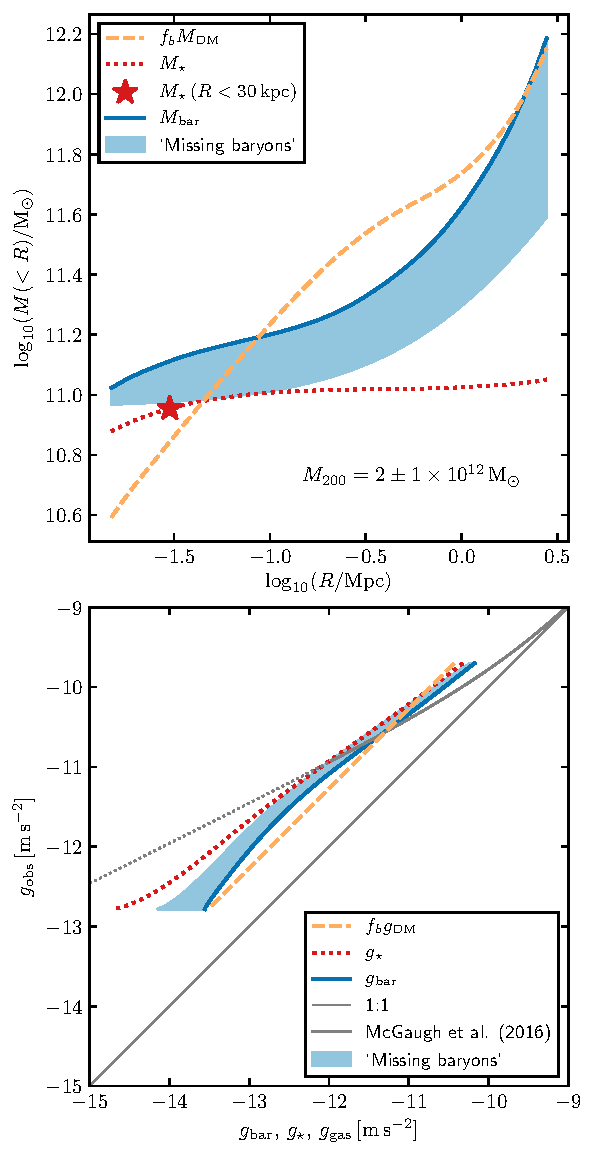
\includegraphics[width=\columnwidth]{Figures/missing_baryons.pdf}
	\caption{\emph{Upper panel: }Cumulative mass profiles of stars (red dotted line) and baryons (dark blue solid line) for BAHAMAS galaxies with $1<M_{200}/(10^{12}\hmsun)<3$. The star marker indicates the stellar mass within a $30\,h^{-1}$~kpc aperture, indicative of what is typically regarded as the stellar mass of a galaxy. The blue shaded band illustrates the difference with the typical baryonic mass profile of observed galaxies of similar mass, estimated based on an extrapolation of the compilation in fig.~7 of \citet{tumlinson2017}. In the inner galaxy the discrepancy between the observed and simulated $M\un{bar}$ is relatively small, but in the outer galaxy the majority of the baryons predicted to be present in BAHAMAS are `missing'. The orange dashed line shows the expected baryonic mass profile if the baryon density is everywhere equal to a fixed fraction $f\un{b}=\Omega\un{b}/\Omega\un{m}$ of the local DM density. At large enough radii ($\gtrsim 2 \hMpc$), the baryon-to-DM ratio converges to the cosmic average. \emph{Lower panel: } As in upper panel, but in acceleration space. The cosmic baryon fraction provides a strong theoretical upper limit on $g\un{bar}$ at low accelerations in the context of the $\lcdm$ cosmology.}
	\label{fig:missing-baryons}
\end{figure}

The calculation of the expected baryonic radial acceleration $g\un{bar}$ requires the enclosed baryonic mass $M\un{bar}(<r)$ within a spherical radius $r$ around the galaxy centre. Since we are dealing with measurements around isolated galaxies at $R>30\hkpc$, we can approximate $M\un{bar}(<r)$ as a point mass $M\un{gal}$ mainly composed of the mass of the lens galaxy itself. $M\un{gal}$ can be subdivided into stars and gas, and the latter further decomposed into cold and hot gas.

The stellar masses of our GAMA and GL-KiDS galaxies are estimated using their multi-band spectral energy distributions, by fitting them with SPS models (see Sect.~\ref{sec:gama} and \ref{sec:gamalike_kids}). The MICE stellar masses are determined from their luminosities using \cite{bell2001} $M/L$ ratios, and the BAHAMAS stellar masses from their calibrated prescriptions for star formation and stellar evolution (see Sect.~\ref{sec:mice_mocks} and \ref{sec:bahamas_mocks}). From these $M_\star$ values, the fraction of cold gas $f\un{cold} = M\un{cold}/M_\star$ can be estimated using scaling relations based on H\,{\sc i} and CO observations. Following \cite{brouwer2017} we use the the best-fit scaling relation found by \cite{boselli2014}, based on the  Herschel Reference Survey \cite[]{boselli2010}:
\begin{equation}\label{eq:fcold}
	\log(f\un{cold}) = -0.69 \, \log(M_\star) + 6.63 \, .
\end{equation}
We apply this equation to all observed and simulated values of $M_\star$ in order to arrive at the total galaxy mass: $M\un{gal} = M_\star + M\un{cold} = M_\star (1 + f\un{cold})$. The spatial distribution of the stellar and cold gas mass are similar \cite[]{pohlen2010,crocker2011,cooper2012,davis2013} and can therefore be considered a single mass distribution, especially for the purposes of GGL which only measures the ESD profile at scales larger than the galaxy disc ($R>30\hkpc$). We illustrate this in Fig.~\ref{fig:missing-baryons}, which shows the enclosed mass profiles (upper panel) and RAR (lower panel) for different baryonic components in the BAHAMAS simulation. The stellar mass within $30 \hMpc$ (red star) gives a good approximation of $M_\star$ across all radii which we consider (dotted red line). We therefore model the baryonic mass of our galaxies as a point mass $M\un{gal}$, containing both the stellar and cold gas mass.

However, the \emph{total} baryonic mass distribution $M\un{bar}$ of galaxies may include a significant amount of additional mass at larger distances, notably in the hot gas phase. This is illustrated in Fig.~\ref{fig:missing-baryons}. In the upper panel, the average baryonic mass profile for BAHAMAS galaxies with $1<M_{200}/(10^{12}\hmsun)<3$ is shown with the blue line. The lower edge of the shaded band corresponds to an estimate of the typical baryonic mass profile for galaxies in the same mass range based on an extrapolation to larger radii of the compilation in \citet{tumlinson2017}, including stars, cold gas ($<10^4\,{\rm K}$, traced by absoption lines such as H\,{\sc i}, Na\,{\sc i} and Ca\,{\sc ii}), cool gas ($10^4$-$10^5\,{\rm K}$, traced by many UV absoption lines, e.g. Mg\,{\sc ii}, C\,{\sc ii}, C\,{\sc iii}, Si\,{\sc ii}, Si\,{\sc iii}, N\,{\sc ii}, N\,{\sc iii}), warm gas ($10^5$-$10^6\,{\rm K}$, traced by C\,{\sc iv}, N\,{\sc v}, O\,{\sc vi} and Ne\,{\sc vii} absoption lines), hot gas ($>10^6\,{\rm K}$, traced by its X-ray emission) and dust (estimated from the reddening of background QSOs, and Ca\,{\sc ii} absorption). The blue shaded region therefore illustrates a component of `missing baryons' predicted by these simulations but not (yet) observed, possibly related to the cosmological missing baryons \citep[e.g.][]{fukugita1998,fukugita2004,shull2012}. There are several possibilities: (i) there may be additional gas present in a difficult-to-observe phase \citep[e.g. hot, low-density gas, see for instance][]{nicastro2018}; (ii) galaxies may eject substantially more gas from their surroundings than is predicted by these simulations; (iii) there may be less baryons in the Universe than expected in the standard cosmology based on big bang nucleosynthesis \cite[BBN,][]{kirkman2003} calculations and CMB measurements \cite[]{spergel2003,planck2014}.

The lower panel of Fig.~\ref{fig:missing-baryons} illustrates the magnitude of the systematic uncertainties in $g_{\rm bar}$. In the $\lcdm$ cosmology, the expectation at sufficiently large radii is given by $g\un{obs}=f^{-1}\un{b} g\un{bar}$ where $f\un{b}$ is the cosmic baryon fraction $f\un{b} = \Omega\un{b}/\Omega\un{m} = 0.17$ \cite[]{hinshaw2013}, shown with the orange dashed line. BAHAMAS, and generically any $\lcdm$ galaxy formation simuation, converges to this line at low enough accelerations (large enough radii). The most optimistic extrapolation of currently observed baryons falls a factor of $\sim 3$ short of this expectation, while the stellar mass alone is a further factor of $\sim 3$ lower. The unresolved uncertainty around these `missing baryons' is the single most severe limitation of our analysis. Given that we are interested in both $\lcdm$ and alternative cosmologies, we will use the galaxy mass $M\un{gal}$ as our fiducial estimate of the total baryonic mass $M\un{bar}$, which is translated into the baryonic acceleration $g\un{bar}$, throughout this work. This serves as a secure lower limit on $g\un{bar}$. \textcolor{black}{We note that the eventual detection, or robust non-detection, of the missing baryons has direct implications for the interpretation of the results presented in Sect.~\ref{sec:results}. We will discuss this issue further in Sect.~\ref{sec:discon}}.

Concerning $g\un{obs}$, omitting the contribution of hot gas will not have a large effect on the prediction within the $\lcdm$ framework (e.g. from simulations) since the total mass distribution at the considered scales is heavily dominated by DM. Within MG frameworks such as EG and MOND, where the excess gravity is sourced by the baryonic matter, it is slightly more complicated. In Sect.~2.2 of \cite{brouwer2017} we carefully modelled the distribution of all baryonic components, based on observations from both GAMA and literature, including their effect on the excess gravity in the EG framework. We found that, for galaxies with $M_\star<10^{11}\hmsun$, the contribution to the ESD profile (and hence to $g\un{obs}$) from hot gas and satellites was small compared to that of the stars and cold gas. Although this analysis was done for the EG theory, the effect of these extended mass distributions within MOND are similar or even less. This allows us to use a point mass $M\un{gal}$ as a reasonable approximation for the baryonic mass distribution $M\un{bar}(<r)$ within our measurement range when computing the predictions of EG and MOND (see Sect.~\ref{sec:EG} and \ref{sec:MOND}).

\subsection{Singular Isothermal Sphere approximation}
\label{sec:SIS_approximation}

When calculating $g\un{obs}$ we start out from our ESD profile measurement, which consists of the value $\Delta\Sigma(R)$ measured in a set of radial bins. At our measurement radii ($R>30\hkpc$) the ESD is dominated by the DM halo. We adopt the simple assumption that our observed density profile $\rho\un{obs}(r)$ is roughly described by a Singular Isothermal Sphere (SIS) model:
\begin{equation}\label{eq:rho_SIS}
	\rho\un{SIS}(r) = \frac{\sigma^2}{2 G \pi r^2} \, . 
\end{equation}
The SIS is generally considered to be the simplest parametrization of the spatial distribution of matter in an astronomical system (such as galaxies, clusters, etc.). It assumes that the dominant constituent particles (in our case DM) behave as an ideal gas that is confined by their combined spherically symmetric gravitational potential, where $\sigma$ is the total velocity dispersion of the particles. The ESD derived from the SIS profile is:
\begin{equation}\label{eq:ESD_SIS}
\Delta\Sigma\un{SIS}(R) = \frac{\sigma}{2 G R} \, .
\end{equation}
From \cite{brouwer2017} we know that, despite its simple form, it provides a good approximation of the WL measurements around isolated galaxies. The SIS profile is therefore well-suited to analytically model the total enclosed mass distribution of our lenses, which can then be derived as follows:
\begin{equation}\label{eq:mass_SIS}
	M\un{SIS}(<r) = 4 \pi \int_{0}^{r}\rho\un{SIS}(r') r'^2 {\rm d} r' = \frac{2\sigma^2 r}{G} \, .
\end{equation}

Now, for each measured value of $\Delta\Sigma\un{obs}$ at its projected radius $R$, we assume that the density profile within $R$ is described by a SIS with $\sigma$ normalized such that $\Delta\Sigma\un{SIS}(R)$ goes through $\Delta\Sigma\un{obs}$. We also assume that we can approximate the spherical distance $r$ with the measured transverse distance $R$. Using these assumptions, we can combine Eqs.~\ref{eq:ESD_SIS} and \ref{eq:mass_SIS} to compute the observed enclosed mass distribution corresponding to that measurement:
\begin{equation}\label{eq:Mobs}
	M\un{obs}(<R) = \frac{2 \, (\Delta\Sigma(R) \, 2 G R) \, r}{G} = 4 \Delta\Sigma(R) \, R^2 \, .
\end{equation}
Through Eq.~\ref{eq:grav}, this results in a very simple expression for the observed gravitational acceleration:
\begin{equation}
g\un{obs}(R) = \frac{G (4 \Delta\Sigma(R) \, R^2)}{r^2} = 4 G \Delta\Sigma(R) \, ,
\end{equation}
computed at each individual point along the ESD profile.

\subsection{Piece-wise power law density profile}
\label{sec:piece-wise_powerlaw}

We can instead assume a self-consistent form for the volume density profile $\rho(r)$ and parametrize it as a piece-wise power law (PPL) constrained to be continuous. This comes at the cost of needing to invert the non-linear function $\Delta\Sigma(\rho)$, which we achieve via an iterative method. We choose to parametrize $\rho(r)$ in terms of $N$ pairs of values $(r_n,\rho_n)$ such that the slope $a_n$ and normalization $b_n$ of the power law profile segments are:
\begin{align}
	\ln\rho &= a_n \ln(r) + b_n \\
	a_n &= \frac{\ln(\rho_{n+1})-\ln(\rho_n)}{\ln(r_{n+1})-\ln(r_n)}\\
	b_n &= \ln(\rho_n) - a_n\ln(r_n)\\
	(a_n, b_n) &=
	\begin{cases}
		(a_0, b_0) & {\rm if}\ r < r_0\\
		(a_n, b_n) & {\rm if}\ r_n \leq r < r_{n+1}\\
		(a_{N-1}, b_{N-1}) & {\rm if}\ r \geq r_N
	\end{cases}
	\label{eq:rho_piecewise_powerlaw}\end{align}
We provide an expression for the discrete ESD profile in terms of the volume density profile, i.e. the function to be inverted, in Appendix~\ref{sec:appendix_invert_esd}.

In order to invert $\Delta\Sigma_m(\rho_n)$, we take as constant the values $R_m$, $\Delta\Sigma_{{\rm obs},m}$ and $r_{n}$. We then propose an initial guess $\rho_n$ which we perturb iteratively, calculating the corresponding $\Delta\Sigma_m$ at each iteration and comparing with $\Delta\Sigma_{{\rm obs},m}$ via the likelihood function:
\begin{align}
	\ln\mathcal{L} &\propto -\frac{1}{2}(\Delta\Sigma\un{obs}-\Delta\Sigma)^{\rm T}C^{-1}(\Delta\Sigma\un{obs}-\Delta\Sigma)
\end{align}
where $C$ is the covariance matrix for the $\Delta\Sigma\un{obs}$. We use the package {\sc emcee} \citep{foreman-mackey13} to estimate the posterior probability distribution of $\rho_n$, and subsequently of the corresponding $g_{{\rm obs},n}$ via integration of the volume density profile.


\subsection{Testing the RAR conversion with BAHAMAS}
\label{sec:conversion_test}

\begin{figure*}
	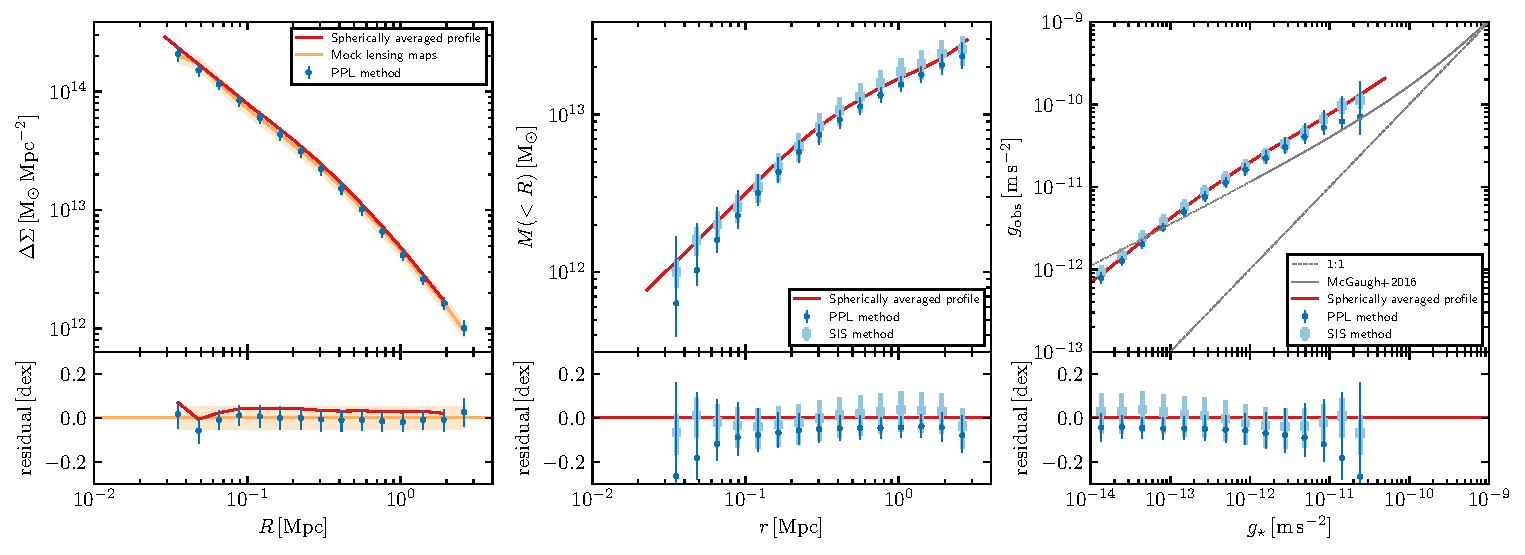
\includegraphics[width=\textwidth]{Figures/compare_method}
	\caption{\emph{Left}: The average ESD profile of a subset of our sample of BAHAMAS galaxies with $10^{13}<M_{200}/(\hmsun)<10^{13.1}$, derived from the spherically averaged mass profile (red line) and the mock lensing maps (yellow line, with an assumed $0.1 \dex$ Gaussian uncertainty). The PPL method recovery of the ESD profile is shown with the blue points; error bars represent 68~per~cent confidence intervals. \emph{Centre}: The SIS (light blue squares) and PPL (blue dots) method recoveries of the spherically averaged enclosed mass profile. The uncertainties on the SIS points are derived by sampling the uncertainties on the mock lensing ESD profile. \emph{Right}: The resulting dynamical acceleration profile $g_{\rm obs}$ and uncertainties, plotted as a function of the acceleration due to stars $g_{\rm star}=GM_\star(<r)/r^2$.}
	\label{fig:compare_method}
\end{figure*}

We now test the accuracy of the two methods outlined in Sects.~\ref{sec:piece-wise_powerlaw} and \ref{sec:SIS_approximation}. As a `test system', we use the $28$ galaxies from our BAHAMAS sample with $10^{13}<M_{200}/(\hmsun)<10^{13.1}$. We combine these into a stacked object by averaging the individual ESD profiles as derived from their mock lensing maps. The stacked ESD as measured from the lensing mocks is shown in the left panel of Fig.~\ref{fig:compare_method} with an orange line. Since the mock ESD profiles are derived from convergence maps (rather than the shapes of background galaxies), they have no associated measurement uncertainty -- for simplicity, we assume a constant $0.1 \dex$ uncertainty, which is similar to that for the KiDS measurements. We also combine the spherically averaged enclosed mass profiles of the galaxies out to $3 \hMpc$ by averaging them. From this average mass profile, we analytically calculate the ESD profile, shown with the red line in the left panel of Fig.~\ref{fig:compare_method}. This line is a near constant $\sim 0.05 \dex$ above that from the lensing mocks, primarily because it does not take into account the additional matter outside the $3\,{\rm Mpc}$ spherical aperture.

The PPL method attempts to reproduce the ESD profile by converging to an appropriate volume density profile. The resulting recovered ESD profile and its 68~per~cent confidence interval is shown with blue points and error bars in the left panel of Fig.~\ref{fig:compare_method} -- the fit to the mock data is excellent. In the centre panel, we show the enclosed mass profile as recovered by both the PPL (dark blue points) and SIS (light blue squares) methods; the true enclosed mass profile is drawn with a red solid line. Both estimators recover the profile within their stated errors. The PPL method systematically underestimates it by $\sim 0.1 \dex$ across most of the radial range. This is directly caused by the difference between the spherically averaged and mock lensing ESD profiles (left panel). The somewhat larger confidence intervals at small radii are caused by the lack of information in the mock data as to the behaviour of the profile at $r < 30 \hkpc$; the model marginalizes over all possibilities. Once the enclosed mass is dominated by the contribution at radii covered by the measurement, the uncertainties shrink.

The SIS method instead slightly underestimates the enclosed mass at small radii, and overestimates it at large radii. The apparent improved performance relative to the PPL method is actually due to a fortuitous partial cancellation of two errors. First, the SIS calculation suffers from the same underestimation of the spherically averaged enclosed mass profile as the PPL method, due to the difference between the mock lensing and spherically averaged ESD profiles. However, in addition to this, the SIS method assumes a density profile $\rho(r)\propto r^{-2}$ at all radii. At small radii, the slope is in reality about $-2.1$. This results in a slight overestimate of the enclosed mass which partially compensates the underestimate described above, resulting in a net underestimate. At larger radii, the slope of the density profile becomes progressively steeper, such that the assumption of an $r^{-2}$ profile increasingly overestimates the enclosed mass, eventually resulting in a net overestimate.

The right panel of Fig.~\ref{fig:compare_method} illustrates the resulting uncertainty in the measurement of the RAR. To focus on the influence of the method used to recover $g\un{obs}$, we simply use the exact spherically averaged stellar mass profile to calculate $g\un{\star}$, plotted on the x-axis\footnote{Note that we do not include the gas, which is predominantly in the hot phase, for consistency with the presentation of the results in Sect.~\ref{sec:results-observables}.}. Both methods yield acceptable estimates of $g\un{obs}$, and we will use both in Sect.~\ref{sec:results-observables} (although after showing that both give consistent measurements, we will show only the SIS measurement to reduce clutter in the figures). We note that the BAHAMAS $g\un{obs}(g\un{\star})$ is significantly offset from the RAR as measured by M16; we will return to this point in Sect.~\ref{sec:results-simulations}.

%The offset between the mock convergence map-derived $\Delta\Sigma$ and the one derived from spherical shells seems to be systematic -- it persists in any BAHAMAS mock sample I choose. The magnitude of the offset seems to vary between about $-0.05 \dex$ and $-0.10 \dex$. I think this depends on the amount of substructure. Imagine a spherically symmetric system and its corresponding surface density map. Now remove a bit of mass from the spherical average and instead put it into a localized substructure at the same radius. The surface density of a few pixels at the location of the substructure will go up a lot, while the surface density of many pixels everywhere else at the same radius will go down a little bit. Depending on how the pixels are combined (more like a median or mean) it's plausible that the case with substructure results in a systematic underestimate of the surface density profile, and therefore the ESD profile.


\subsection{Testing the RAR conversion with KiDS-1000: lensing rotation curves}
\label{sec:results-rotation}

%Plot: KiDS-1000 lensing rotation curves
\begin{figure*}
	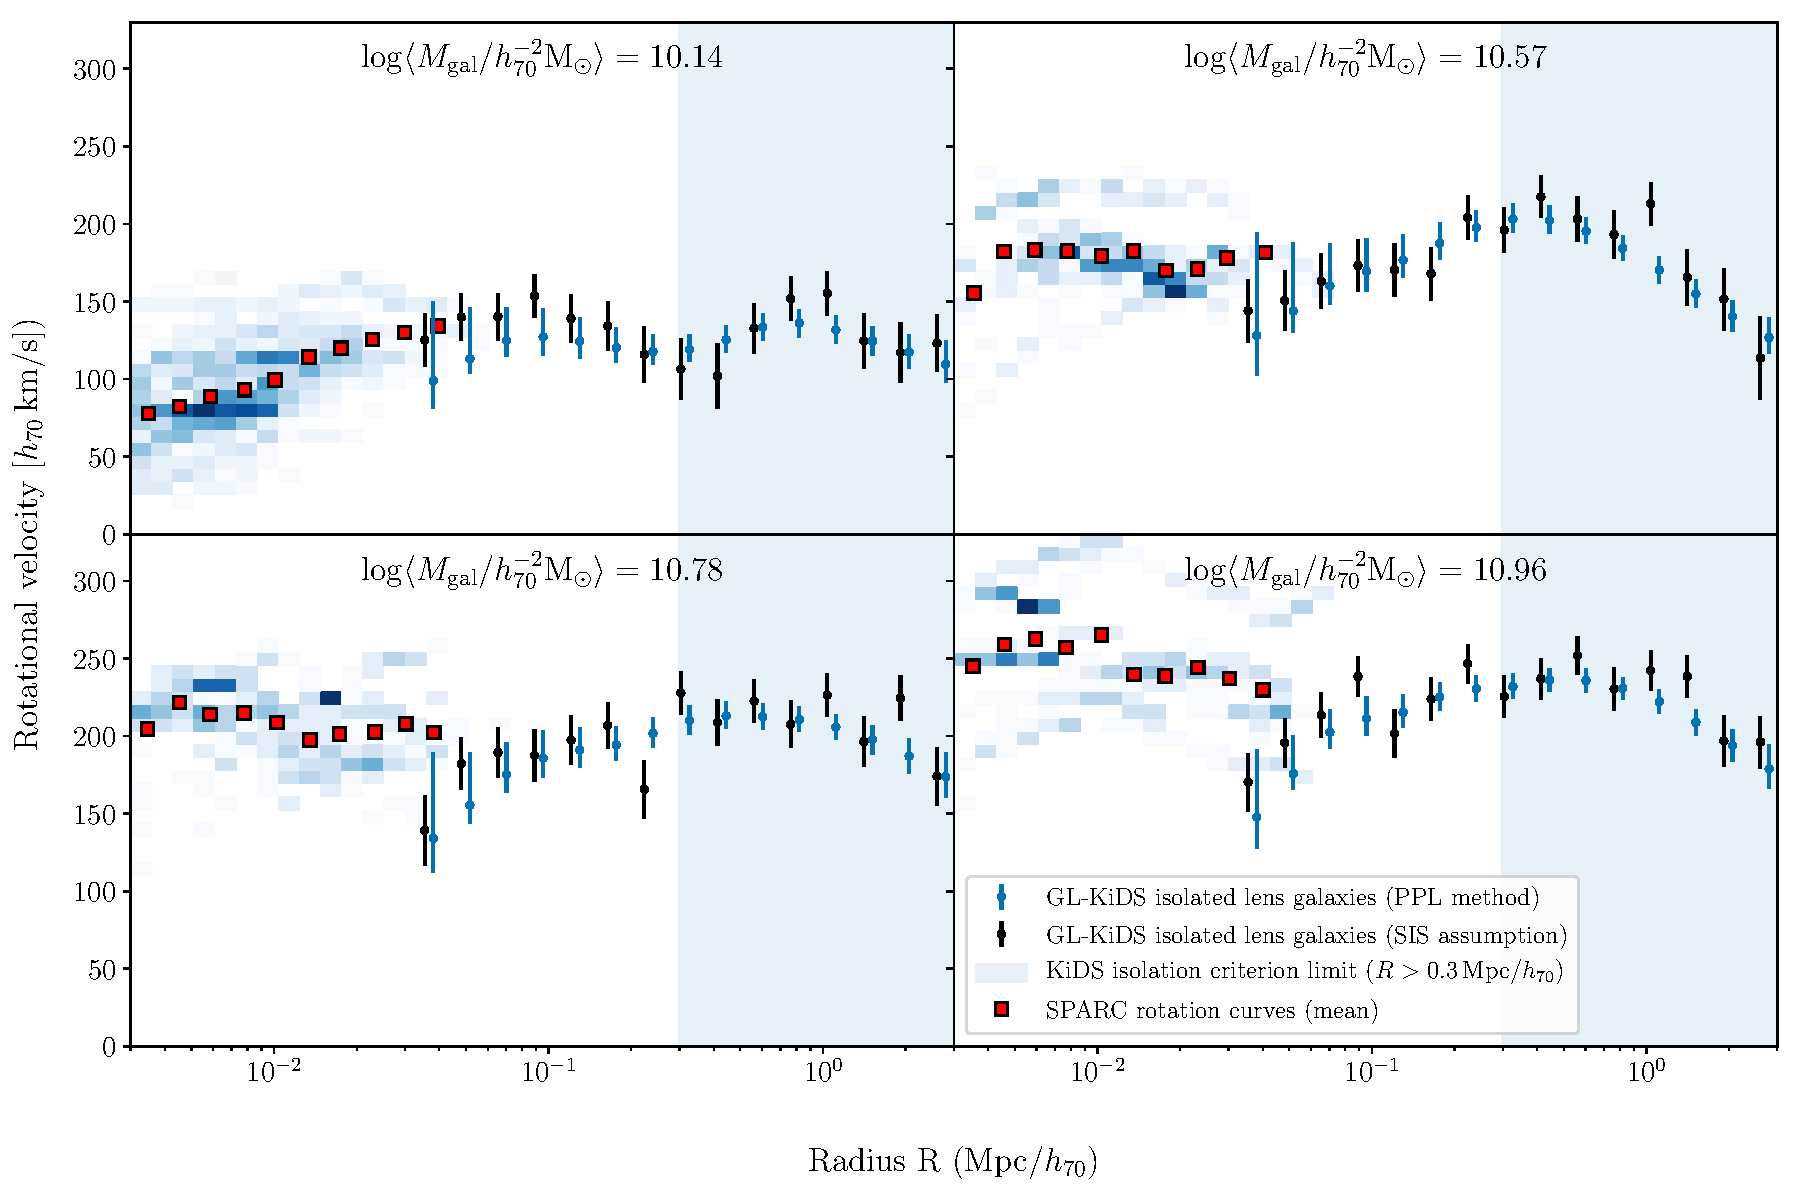
\includegraphics[width=\textwidth]{Figures/ESD_KiDS_massbins-8p5_10p3_10p6_10p8_11p0_iso.pdf}
	\caption{Lensing rotation curves, the rotational velocity as a function of radius $v\un{rot}(R)$, measured using the GL-KiDS isolated lens sample divided into 4 stellar mass bins. The black dots (with $1\sigma$ error bars) show the result calculated using the SIS assumption, while the blue dots (with error bars representing the 16th and 84th percentile of the fits) show the result from the more sophisticated PPL method. Our measurements are consistent between the two methods, and also with the rotation curves from SPARC (all data as the blue 2D histogram, the mean as red squares).}
	\label{fig:Vrot_kids_verlinde_mice}
\end{figure*}

As a final consistency check between the SIS assumption and the PPL method, we apply both methods to the true KiDS-1000 data. Since these methods are only used to convert $\Delta\Sigma(R)$ into $g\un{obs}(r)$, we can leave $g\un{bar}$ out of the comparison and plot our results as a function of $R$. An observable closely related to the RAR that is usually plotted as a function of radius, is the traditional rotation velocity curve:
\begin{equation}\label{eq:Vrot}
v\un{rot}(r) = \sqrt{\frac{G M\un{obs}(<r)}{r}} \, ,
\end{equation}
which indeed served as input to the M16 RAR measurement. We can very simply apply the same SIS method described in Sect.~\ref{sec:SIS_approximation} to convert our ESD profiles $\Delta\Sigma(R)$ into $v\un{rot}(R)$, since substituting Eq. \ref{eq:Mobs} into Eq. \ref{eq:Vrot} gives:
\begin{equation}
v\un{rot}(R) = \sqrt{\frac{G \, (4 \Delta\Sigma(R) \, R^2)}{r}} \, = \sqrt{4 G \, \Delta\Sigma(R) \, R} \, .
\end{equation}
Just as easily, Eq. \ref{eq:Vrot} can be used to compute $v\un{rot}(R)$ from the $M(<R)$ calculated through the PPL method described in Sect.~\ref{sec:piece-wise_powerlaw}.

Fig.~\ref{fig:Vrot_kids_verlinde_mice} shows the lensing rotation curves for isolated GL-KiDS galaxies, divided into 4 stellar mass bins using the following limits: $\log_{10}(M_\star/\hmsun) = [8.5,10.3,10.6,10.8,11.]$. Showing the data in this way allows us to observe (for the first time in this intuitive manner) how rotation curves of isolated galaxies continue beyond the observable disc ($r>30\hkpc$). In addition, it provides a consistency check with the SPARC rotation curves \cite[]{lelli2016b} which form the basis for the M16 RAR measurement. It is remarkable how well the mean of the SPARC rotation curves and our lensing results correspond at their intersection ($r\sim 30 \hkpc$). But most importantly, we find that the rotation curves from the SIS assumption (black dots with $1\sigma$ error bars) are consistent with the ones from the PPL method (blue dots with error bars showing the 16th and 84th percentile of the fits). Although the SIS assumption results in slightly more scatter, there is very little systematic bias between the results from the two methods, which have a fractional difference of $\meanb{\log(v\un{rot, SIS} / v\un{rot, PPL})} = 0.017 \dex$. Since this measurement is merely a different way of presenting the observed acceleration, which equals $g\un{obs}(r) = v\un{rot}^2 / r$, we can easily compute that the expected difference in $g\un{obs}$ would be $\meanb{\log(g\un{obs, SIS} / g\un{obs, PPL})} = 0.038 \dex$.

The consistency between the two conversion methods allows us to use the SIS assumption throughout this work. The great advantage of this method is that it allows us to convert GGL profiles binned by baryonic acceleration $\Delta\Sigma(g\un{bar})$, into the RAR: $g\un{obs}(g\un{bar})$. This is not the case for the PPL method, which only works on $\Delta\Sigma(R)$ binned by radius. The former can therefore be applied to any lens sample; the latter only to lenses within a narrow mass range (in order to convert $R$ into $g\un{bar}$ using the mean $\meanb{M\un{gal}}$). To account for the added uncertainty resulting from the conversion to the RAR, we add $0.1 \dex$ to the error bars of our RAR measurements throughout this work.

\begin{comment}
same lensing results already shown in Fig.~\ref{fig:RAR_kids_mice_mstarbins}

Without doubt the RAR, as a direct comparison of the expected versus the total gravitational fields, has proven to be a valuable tool in testing DM and MG models. However, one fundamental limitation to RAR measurements at large scales remains that we do not have reliable observations of individual galaxies' hot gas and `missing baryon' contributions to $g\un{bar}$. Instead we use $M\un{gal}$ to estimate $g\un{bar}$, which means that our measurements are very sensitive to systematic biases in the stellar mass measurements, which can be as high as $0.2 \dex$. Although these limitations are elaborately discussed in Sect.~\ref{sec:baryonic_mass} and taken into account in all results in Sect.~\ref{sec:results}, it is valuable to seek tests that circumvent them.

One possibility explored by \cite{oman2020} is to invert the empirical relation from M16. At high accelerations Eq. \ref{eq:rar_mcgaugh} corresponds to $g\un{bar} \propto g\un{obs}^2$ which, using Newton's gravitational law (Eq. \ref{eq:grav}) can be converted into the cumulative baryonic mass:
\begin{equation}
M\un{bar}(<r) \propto  \left( \frac{M\un{obs}(<r)}{r} \right)^2 \, .
\end{equation}
Because this mass is cumulative, it must comply to ${\rm d}M\un{bar}(r)/{\rm d}r > 0$ to avoid the need for negative baryonic mass. This means that necessarily ${\rm d}M\un{obs}(r)/{\rm d}r > 1$, which corresponds to a density profile with a slope no steeper than $\rho\un{obs} \propto r^{-2}$. \cite{oman2020} explore various large-scale measurements of $\rho\un{obs}(r)$ to look for evidence that suggests a steeper slope, which would pose a problem for MOND if found within it's regime of validity\footnote{The regime where MOND predictions are valid depends primarily on the External Field Effect.}. Although they find tentative hints to a declining slope, more data is needed to determine whether the evidence is significant.
\end{comment}

\section{Theoretical predictions}
\label{sec:theories}

\subsection{Modified Newtonian Dynamics}
\label{sec:MOND}

With his theory of Modified Newtonian Dynamics (MOND), \cite{milgrom1983} postulated that the `missing mass problem' in galaxies is not caused by an undiscovered fundamental particle, but that instead our current gravitational theory should be revised. MOND's basic premise is that one can adjust Newton's second law of motion ($F=ma$) by inserting a general function $\mu(a/a_0)$, which only comes into play when the acceleration $a$ of a test mass $m$ is much smaller than a critical acceleration $a_0$. This function predicts the observed flat rotation curves in the outskirts of galaxies, while still reproducing the Newtonian behaviour of the inner disc. In short, the force $F$ becomes:
\begin{align}\label{eq:mond_f}
	& F(a) = m \, \mu(\frac{a}{a_0}) \, a \, ,
	& \mu(x \gg 1) \approx 1 \, , \, \mu(x \ll 1) \approx x \, .
\end{align}
This implies that $a\gg a_0$ represents the Newtonian regime where $F\un{N} = m \, a\un{N}$ as expected, while $a\gg a_0$ represents the `deep-MOND' regime where $F\un{dM}=m \, a\un{dM}^2/a_0$. In a circular orbit, this is reflected in the deep-MOND gravitational acceleration $g\un{dM} \equiv a\un{dM}$ as follows:
\begin{align}\label{eq:mond_g}
	& F\un{dM} = m \frac{a\un{dM}^2}{a_0} = \frac{G \, M m}{r^2}
	& \rightarrow \,  g\un{dM} = \sqrt{a_0 \frac{G M}{r^2}} \, .
\end{align}
This can be written in terms of the expected baryonic acceleration $g\un{bar}=GM/r^2$ as follows:
\begin{equation}
	g\un{dM}(g\un{bar}) = \sqrt{a_0 \, g\un{bar}} \, ,
\end{equation}
which demonstrates that MOND predicts a very simple relation for the RAR: $g\un{obs}=g\un{bar}$ in the Newtonian regime ($g\un{obs}\gg a_0$), and following Eq. \ref{eq:mond_g} in the deep-MOND regime ($g\un{obs}\ll a_0$). However, since $\mu(a/a_0)$, also known as the `interpolating function', is not specified by \cite{milgrom1983}, there is no specific constraint on the behaviour of this relation in between the two regimes. In the work of \cite{milgrom2008}, several families of interpolation functions are discussed. Selecting the third family (given by their eq.~13) with constant parameter $\alpha=1/2$, provides the function that M16 later used to fit to their measurement of the RAR using rotation curves of $153$ galaxies. This relation can be written as:
\begin{equation}\label{eq:rar_mcgaugh}
	g\un{obs} = \frac{g\un{bar}}{1 - e^{-\sqrt{g\un{bar}/a_0}}} \, ,
\end{equation}
where $a_0 \equiv g\un{\dagger}$ corresponds to the fitting parameter constrained by M16 to be $g\un{\dagger}=1.20\pm0.26\E{-10} \mpss$. Since Eq. \ref{eq:rar_mcgaugh} (equal to eq. 4 in M16) is also considered a viable version of the MOND interpolation function by \cite{milgrom2008}, we will consider it the baseline prediction of MOND in this work. As the baseline value of $a_0$, we will likewise use the value of $g\un{\dagger}$ measured by M16, since it exactly corresponds to the value of $a_0=1.2\E{-10} \mpss$ considered canonical in MOND since it's first measurement by \cite{begeman1991}, using the rotation curves of 10 galaxies.

Since the MOND theory described above is a non-relativistic (NR) theory, performing WL measurements to test it requires the assumption that light is curved by a MONDian gravitational potential in the same way as in GR. This assumption is justified since \citet[][while testing the MOND paradigm using GGL data from the Canada-France-Hawaii Telescope survey]{milgrom2013} states that NR MOND is a limit of relativistic versions, which predict that gravitational potentials determine lensing in the same way as Newtonian potentials in GR.

\subsection{Emergent Gravity}
\label{sec:EG}

The work of \citet[][V16 hereafter]{verlinde2016}, which is embedded in the framework of string theory and holography, shares the view that the missing mass problem is to be solved through a revision of our current gravitational theory. Building on the ideas of \cite{jacobson1995,jacobson2016,padmanabhan2010,faulkner2015} and his own previous work \cite[]{verlinde2011}, V16 abandons the notion of gravity as a fundamental force. Instead, it emerges from an underlying microscopic description of space-time, in which the notion of gravity has no \emph{a priori} meaning.

The aforementioned earlier works have shown that constructing an EG theory in a static (`anti-de Sitter') universe allows for the re-derivation Einstein's laws of GR. A distinguishing feature of V16 is that it attempts to describe an expanding (`de Sitter') universe which is filled with a DE component. This results in a new volume law for gravitational entropy caused by DE, in addition to the area law normally used to retrieve Einsteinian gravity. According to V16, energy that is concentrated in the form of a baryonic mass distribution causes an elastic response in the entropy of the surrounding DE. This results in an additional gravitational component at scales set by the `Hubble acceleration scale' $a\un{0} = c H_0/6$. Here $c$ is the speed of light, and $H_0$ is the current Hubble constant which measures the Universe's expansion velocity.

Because this extra gravitational component is predicted to explain the effects usually attributed to DM, it is conveniently expressed as an \emph{apparent} dark matter (ADM) distribution:
\begin{equation}
M\un{D}^2 (r) = \frac{  cH_0 r^2}{6G} \frac{d\left( M\un{bar}(r) r \right)}{dr} \, .
\label{eq:veg_mdm}
\end{equation}
Thus the ADM distribution is completely defined by the baryonic mass distribution $M\un{bar}(r)$ as a function of the spherical radius $r$, and a set of known physical constants.

Since we measure the ESD profiles of galaxies at projected radial distances $R>30 \hMpc$, we can assume that their baryonic component is enclosed within the minimal measurement radius \cite[see also][]{brouwer2017}. This is equivalent to describing the galaxy as a point mass $M\un{bar}$, which allows us to simplify Eq. \ref{eq:veg_mdm} to:
\begin{equation}
M\un{D}(r)=\sqrt{\frac{cH_{0} \, M\un{bar}}{6 \, G}} \, r \, .
\end{equation}
Now the total enclosed mass, $M\un{EG}(r) = M\un{bar} + M\un{D}(r)$, can be used to calculate the predicted gravitational acceleration $g\un{EG}(r)$ as follows:
\begin{equation}
	g\un{EG}(r) = \frac{G M\un{EG}(r)}{r^2} = \frac{G M\un{bar}}{r^2} + \sqrt{\frac{cH_{0}}{6}} \, \frac{\sqrt{G M\un{bar}}}{r} \, .
\end{equation}
In terms of the expected baryonic acceleration $g\un{bar}(r) = G M\un{bar}/r^2$, this simplifies even further to:
\begin{equation}
\label{eq:rar_verlinde}
g\un{EG}(g\un{bar}) = g\un{bar} + \sqrt{\frac{cH_{0}}{6}} \, \sqrt{g\un{bar}} \, .
\end{equation}

Note that Eq. \ref{eq:veg_mdm} is only a macroscopic approximation of the underlying microscopic phenomena described at the start of this section, and is thus only valid for static, spherically symmetric and isolated baryonic mass distributions. For this reason, we select only the most isolated galaxies from our sample (see Sect.~\ref{sec:isolation}), such that our WL measurements are not unduly influenced by neighbouring galaxies. In addition, cosmological evolution of the $H_0$ parameter is not yet implemented in the theory, restricting its validity to galaxies with relatively low redshifts. However, we calculate that at our mean lens redshift ($\langle z \rangle \sim 0.2$) using an evolving $H(z)$ would result in only a $\sim5$~per~cent difference in our ESD measurements, based on the background cosmology used in this work.

In order to test V16 using the standard WL methodology, we need to assume that the deflection of photons by a gravitational potential in this alternative theory corresponds to that in GR. This assumption is justified because, in EG's original (anti-de Sitter) form, Einstein's laws emerge from its underlying description of space-time. The additional gravitational force described by ADM does not affect this underlying theory, which is an effective description of GR. Therefore, we assume that the gravitational potential of an ADM distribution produces the same lensing shear as an equivalent distribution of actual matter.

\subsection{Analytical CDM model}
\label{sec:analytical}

To help guide an intuitive interpretation of the lensing RAR within the framework of the $\lcdm$ theory, we make use of the simple model of N17 which combines a basic model of galactic structure and scaling relations to predict the RAR. We refer to N17 for a full description, but give a summary here. A galaxy of a given stellar (or baryonic -- there is no distinction in this model) mass occupies a DM halo of a mass fixed by the abundance matching relation of \citet{behroozi2013}. The dark halo concentration is fixed to the cosmological mean for haloes of that mass \citep{ludlow2014}. The baryonic disc follows an exponential surface density profile with a half-mass size fixed to $0.2\times$ the scale radius of the dark halo (N17). The above is sufficient to specify the cumulative mass profile of both the baryonic and dark components of the model galaxy; calculating $g\un{obs}$ and $g\un{bar}$ is then straightforward.


\section{Results: the RAR of isolated galaxies}
\label{sec:results}

We apply the isolation criterion ($r\un{sat}(f\un{M_\star}>0.1)>3\hMpc$, see Sect.~\ref{sec:isolation}) to the lens galaxy samples, measure their ESD profiles (Sect.~\ref{sec:lensing}) and convert these into the RAR (Sect.~\ref{sec:conversion}). The same procedure is applied to the mock lens samples from MICE and BAHAMAS in order to obtain the prediction from $\lcdm$ simulations, while the predictions from MOND, EG and the N17 CDM model are calculated analytically based on the average baryonic mass of each lens galaxy (sub)sample. In the following three sections, we show the results of the lensing RAR measurements and compare these to the respective predictions. In this section we concentrate on the results from the full isolated galaxy sample, and compare it to the predictions of the analytical models described in Sect.~\ref{sec:analytical}: MOND, EG and the $\lcdm$-based N17 model, and the MICE and BAHAMAS simulations described in Sects.~\ref{sec:mice_mocks} and \ref{sec:bahamas_mocks}.


\subsection{Comparison to Modified Gravity theories}
\label{sec:results-analytical}

%Plot: GAMA + KiDS + EG (isolated)
\begin{figure*}
	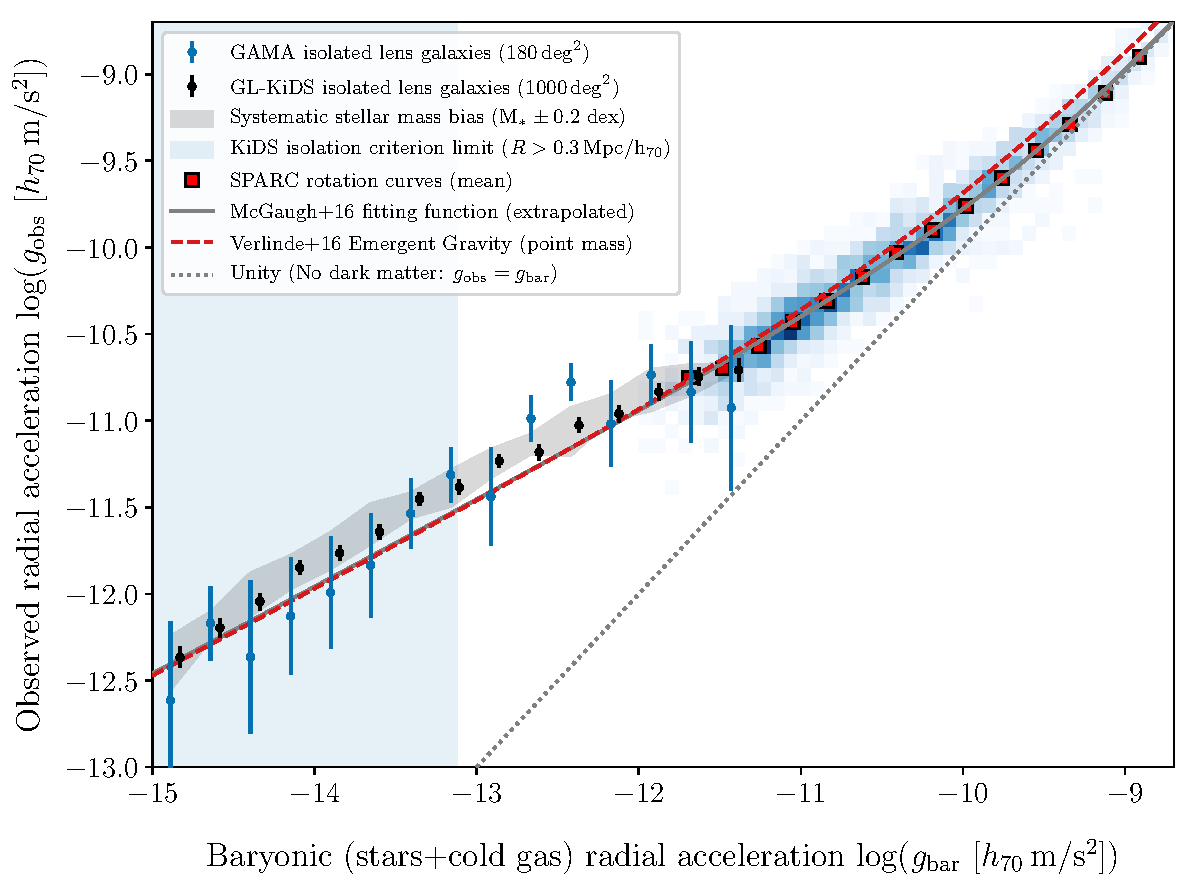
\includegraphics[width=0.8\textwidth]{Figures/RAR_KiDS+GAMA+Verlinde_Nobins_isolated_zoomout.pdf}
	\caption{The RAR is defined as the measured total gravitational acceleration $g\un{obs}$ (y-axis) and the expected baryonic acceleration $g\un{bar}$ (x-axis) of galaxies. At high accelerations (corresponding to small scales) we show the M16 RAR measurements from galaxy rotation curves (all data as the blue 2D histogram, the mean as red squares). Using weak gravitational lensing we are able to extend this measurement to lower accelerations, using both the spectroscopic GAMA and the photometric GL-KiDS isolated lens samples (dark blue and black dots with $1\sigma$ error bars). Comparing our lensing observations to two MG models: MOND (the M16 fitting function; grey solid line) and EG (assuming a point mass; red dashed line) we find that GAMA results are in agreement with the two models, while those from GL-KiDS seem systematically higher. However, especially at very low accelerations (corresponding to $R > 0.3 \hMpc$, light blue shaded region) the uncertainty in the photometric KiDS redshifts affects the isolated lens selection, resulting in systematically higher values of $g\un{obs}$ due to the possible contribution of satellites. In addition, the tension could be relieved by the systematic stellar mass uncertainty ($\Delta M_\star=0.2 \dex$, grey band).}
	\label{fig:RAR_kids_gama_verlinde}
\end{figure*}

In Fig.~\ref{fig:RAR_kids_gama_verlinde} we show the RAR, with the `observed radial acceleration' computed from our lensing measurements on the y-axis. The x-axis shows the expected `baryonic (star+cold gas) radial acceleration', where the label serves as a reminder that throughout this work $g\un{bar}$ is only computed from the measured stellar masses of the galaxies and an estimate of their cold gas component (see Sect.~\ref{sec:baryonic_mass}). The fact that we cannot incorporate the \emph{total} baryonic mass distribution into our comparison, including the hot gas and a possible `missing baryon' contribution, remains a fundamental limitation to all works testing DM/MG theories at large scales. As shown in Fig.~\ref{fig:missing-baryons}, these difficult to observe components can have a very large effect on the horizontal positions of the data-points. However, we can safely continue as long as \emph{all} estimates of $g\un{bar}$ (in the measurements, models and simulations) are based only on these same components (stars+cold gas), as mentioned in Sect.~\ref{sec:baryonic_mass}. In that same section, we established that the $g\un{obs}$ prediction of the MG models tested here are not altered much by including extended baryonic components such as hot gas.

The dark blue and black points with $1\sigma$ errors show $g\un{obs}$ measured using the GAMA and GL-KiDS isolated lens samples respectively. Due to its smaller survey area ($180$ vs. $1006 \deg^2$), the error bars using GAMA lenses are larger than those using GL-KiDS lenses. However, as explained in Sect.~\ref{sec:isolation}, the spectroscopic redshifts of the GAMA survey allow for a much more reliable selection of the isolated lenses compared to KiDS (which measures photometric redshifts with a $\sigma\un{z}=0.02$ uncertainty). The effect of this uncertainty on the measured lensing profiles is modelled in Fig.~\ref{fig:isolation_test_offset}, which shows that the ESD profile of the `offset' MICE sample diverges from the truly isolated MICE galaxies at radius $R > 0.3 \hMpc$. At these large scales, the effect of satellite galaxies on the lensing signal result in $\sim30$~per~cent higher values of $\Delta\Sigma$ due to the contribution of satellite galaxies. We translate this radius into a gravitational acceleration value using Eq. \ref{eq:grav}, based on the average $M\un{gal}$ of the lens sample. In this way we estimate that, for the full sample of isolated GL-KiDS galaxies, the isolation criterion is no longer reliable when $g\un{bar} \lessapprox 10^{-13} \mpss$, as indicated by the light blue shaded region. Note that the GAMA results, which are based on accurate spectroscopic redshift measurements, are still valid within this region.

The grey band shows the range of possible bias due to a $\Delta M_\star=0.2 \dex$ systematic shift in stellar mass. We estimate this range by performing our analysis assuming stellar masses that are $0.2 \dex$ higher/lower than their best-fitting $M_\star$ values (see Sect.~\ref{sec:gamalike_kids}). We only show this band once, for the GL-KiDS result, but note that this bias equally affects the GAMA stellar masses (and, indeed, any stellar mass measurement; see \citealt{wright2017}).

Alongside our results we show the M16 RAR measurements (both the full dataset: blue 2D histogram, and the mean: red squares), from SPARC galaxy rotation curves, which cover higher accelerations than our lensing measurements (corresponding to smaller scales: $R < 30 \hkpc$). At the highest acceleration end (smallest scales), where $g\un{obs}$ is dominated by $g\un{bar}$, they follow a one-to-one relation (grey dotted line). At lower accelerations (larger scales) their results quickly diverge from unity, signifying the start of the DM dominated regime. It is very reassuring that, although we use completely different methods to measure the RAR, our results overlap perfectly between $10^{-12} < g\un{bar} < 10^{-11} \mpss$ (corresponding to $R \sim 30 \hkpc$). In this work we compare the two MG models, EG (red dashed line) and MOND (grey solid line), only to our lensing results (for a comparison of these two models with the RAR from SPARC, see \citealt{lelli2017a}). As explained in Sect.~\ref{sec:MOND}, we take the MOND prediction to be equal to the extrapolated M16 fitting function (Eq. \ref{eq:rar_mcgaugh}), and that of EG as the prediction from \cite{verlinde2016} for a point mass (Eq. \ref{eq:rar_verlinde}). Within our measurement range, the two predictions are almost indistinguishable. Both models appear to be compatible with the GAMA data, while the GL-KiDS data-points lie systematically above the predictions. However, this could be caused by the contribution of satellites due to the mentioned uncertainty in the photometric GL-KiDS redshifts, especially at accelerations $g\un{bar} < 10^{-13} \mpss$. The mentioned $0.2 \dex$ stellar mass bias can also alleviate this tension (but only if it happens to be in the right direction).

To quantify our findings, we compare the acceleration predicted by the model $g\un{mod}$ with the observed $g\un{obs}$ by calculating the $\chi^2$ value:
\begin{equation}
\chi^2 = (g\un{obs} - g\un{mod})^\intercal \cdot C^{-1}(g\un{obs} - g\un{mod}) \, ,
\label{eq:chi2}
\end{equation}
where $C^{-1}$ is the inverse of the analytical covariance matrix (see Sect.~\ref{sec:lensing}). We divide this quantity by the number of degrees of freedom $N\un{DOF}$ of the model, which gives us the reduced $\chi^2$ statistic:
\begin{equation}
\chi\un{red}^2 = \frac{\chi^2}{N\un{DOF}} = \frac{\chi^2}{N\un{data} - N\un{param}} \, ,
\end{equation}
Here $N\un{data}$ is the number of data-points in the measurement and $N\un{param}$ is the number of free parameters in the model. Since none of the models have free parameters, $N\un{DOF}$ is simply the total number of $g\un{bar}$-bins (in this case $N\un{data}= 15$).

Comparing the GAMA data to the two MG models results in $\chi\un{red}^2$-values of $0.81$ for MOND and $0.82$ for EG, corresponding to a standard deviation of $0.43$ and $0.45 \sigma$ respectively. This confirms that both models agree well with the GAMA data, with a slight advantage for the MOND prediction. When using the GL-KiDS results, both models perform much worse: $\chi\un{red}^2=5.20$ and $5.69$ for MOND and EG respectively, corresponding to $>6 \sigma$ standard deviations. Taking into account the effect of the photo-z uncertainty of GL-KiDS by only using the $7$ data-points within the isolation criterion limit ($R < 3 \hMpc$) results in slightly better values: $\chi\un{red}^2 = 25.79/7 = 3.46$ for MOND and $\chi\un{red}^2 = 27.55/7 = 3.94$ for EG, although this is still $\sim3.5 \sigma$ away from a good fit. Of course there is still the possible $\Delta M_\star = 0.2 \dex$ bias in stellar mass, shown by the grey band. If this would shift the data downward, the $\chi\un{red}^2$ of MOND (or similarly for EG) could be as low as $1.45$ (with the data-points beyond the isolation criterion limit still removed). If it shifts the data upward, however, this $\chi\un{red}^2$ could be as high as $14.93$. Thus, although the MOND and EG predictions are able describe our measurements within the statistical and systematic uncertainties, whether these models are confirmed or excluded relies heavily on the the systematic bias in the stellar mass measurements. This highlights the general point that GGL measurements are now so accurate in determining the total observed mass distribution that improving the RAR measurement depends primarily on getting a better handle on the baryonic mass distribution.

\subsection{Comparison to the N17 analytical model}

%Plot: KiDS + Navarro
\begin{figure*}
	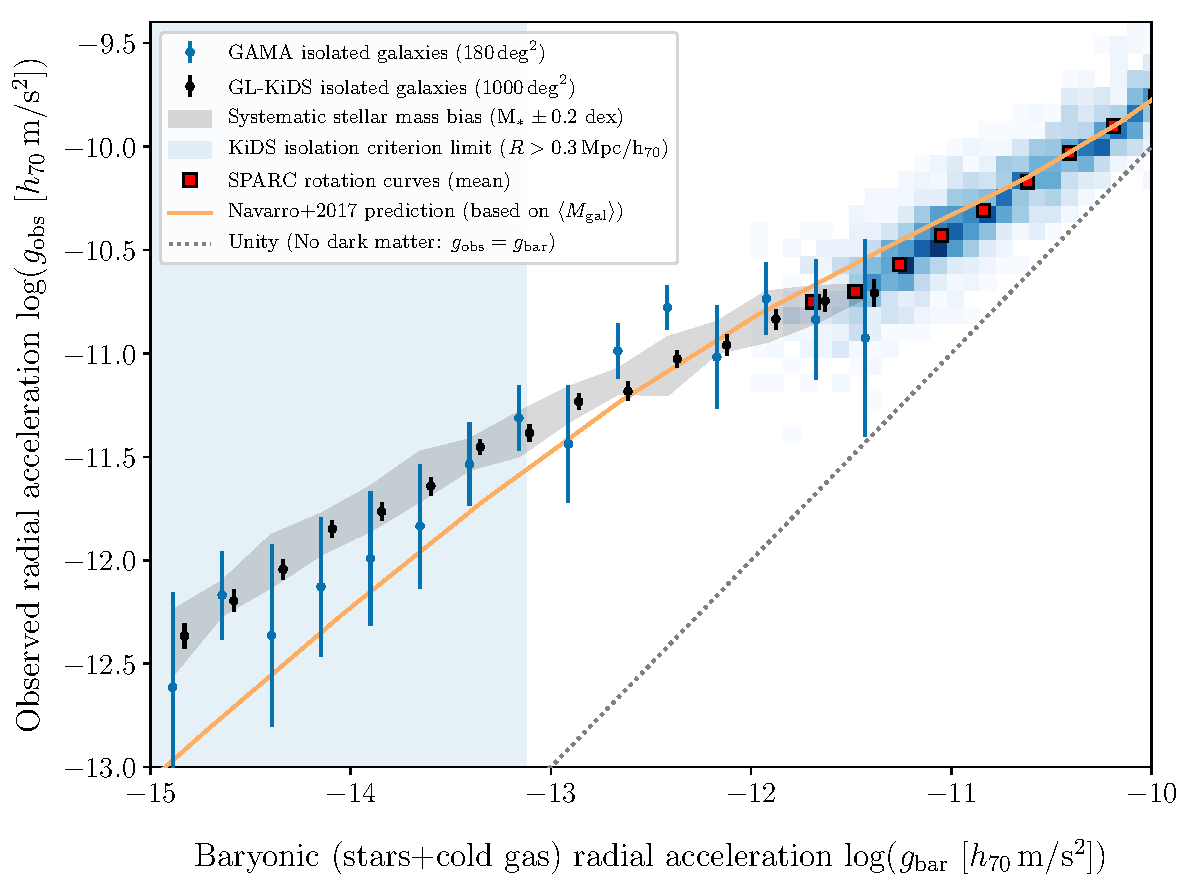
\includegraphics[width=0.8\textwidth]{Figures/RAR_KiDS+GAMA+Navarro_Nobins_isolated.pdf}
	\caption{The RAR measured using the spectroscopic GAMA and the photometric GL-KiDS isolated lens samples (dark blue and black dots with $1\sigma$ error bars). We compare our results to the analytical $\lcdm$-based model created by N17. At higher accelerations there is a good match between the N17 model and the M16 observations, as expected. However, at lower accelerations the model bends down with respect to the lensing measurements, due to the steep outer slope of the NFW density profile ($\rho \propto r^{-3}$). Large-scale contributions to the total mass distribution, such as the average cosmic DM density, could slightly mitigate this discrepancy. However, these are not implemented into the simple analytical N17 model, which was created to reproduce the RAR at the small scales measured by rotation curves.}
	\label{fig:RAR_kids_gama_Navarro}
\end{figure*}

The final analytical prediction we test is the $\lcdm$-based model created by N17. In Fig.~\ref{fig:RAR_kids_gama_Navarro} we show the RAR predicted by this model for a galaxy with a baryonic mass equal to the average stellar + cold gas mass of the lens sample ($\log_{10}\meanb{M\un{gal}} = 10.89$). We compare this prediction to the same observations as shown in Fig.~\ref{fig:RAR_kids_gama_verlinde}. Although we still show the M16 RAR measurements from galaxy rotation curves for reference, we zoom in on the lower accelerations that are the focus of this work. At higher accelerations there is a good match between the model and the M16 RAR measurements from galaxy rotation curves, which is expected since the model is designed and confirmed to reproduce these results in the N17 paper. However, at the lower accelerations unique to our lensing measurements the predicted $g\un{obs}$ bends up and then down compared to our measurements. Due to its large error bars, the GAMA data can still accommodate the analytical prediction: $\chi\un{red}^2 = 13.96 / 15 = 0.93$. The GL-KiDS result, even with all data-points beyond the KiDS isolation limit ($R>3 \hMpc$) removed, excludes the N17 prediction with $\chi\un{red}^2 = 31.67 / 7 = 4.52$, corresponding to $4.07 \sigma$.

The strong downward slope results from the $r^{-3}$ radial dependence of the NFW density profile at large scales (where an $r^{-2}$ density profile would instead follow the same slope as the MG predictions in Fig.~\ref{fig:RAR_kids_gama_verlinde}). This effect could be slightly mitigated by taking into account the average DM density of the Universe, which would result in an upwards turn towards an $r^{-1}$ slope at $g\un{bar}>10^{14}$ (as shown by the BAHAMAS prediction of the RAR in the lower panel of Fig.~\ref{fig:missing-baryons}). However, components contributing to the large-scale DM profile are not implemented into the N17 model, which was created to reproduce the RAR at the small scales measured by rotation curves. It is clear from this exercise that, while succeeding to describe the RAR at small scales, this simple model is not sufficient to reproduce the results at the larger scales probed by weak lensing. This requires more elaborate modelling within the $\lcdm$ paradigm, represented by large cosmological simulations such as BAHAMAS and MICE. In the next section (Sect.~\ref{sec:results-simulations}) we will make a more fair comparison using these two simulations, which can mimic the measurement more faithfully.

%Kyle: I think the focus in this section should actually be that the N17 model makes a very different prediction, and actually does it reasonably well. Where is struggles most is when the cosmological background density starts to kick in, which forces the curve back toward a slope of -1, as in Fig.~1 of my rejected draft. Including more baryons in this model just makes the discrepancy with the lensing worse as the curve shifts further right. Can end by saying that this initial impression turns out to be wrong, and we will explain why by making a more fair comparison using MICE and BAHAMAS where we can mimic the measurement more faithfully.

\subsection{Comparison to $\lcdm$ simulations}
\label{sec:results-simulations}

%Plot: KiDS + BAHAMAS + MICE (isolated)
\begin{figure*}
	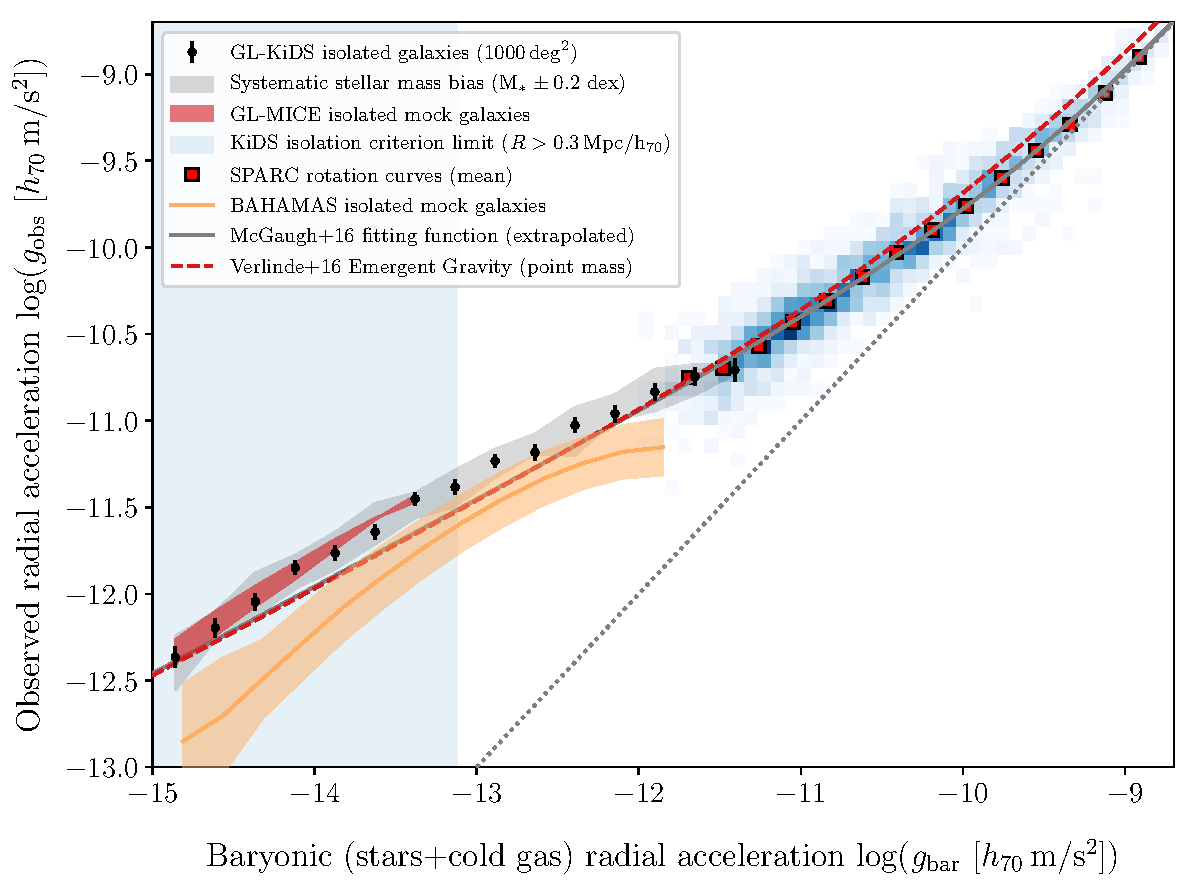
\includegraphics[width=0.8\textwidth]{Figures/RAR_KiDS+MICE+Bahamas+Verlinde_No_Nobins_isolated_zoomout.pdf}
	\caption{The RAR measured using the spectroscopic GAMA and the photometric GL-KiDS isolated lens samples (dark blue and black dots with $1\sigma$ error bars) compared to two $\lcdm$ simulations. The BAHAMAS results (orange band) reflect the median and $16^{\rm th}$ and $84^{\rm th}$ percentiles of the simulated lens galaxies, while the MICE results (red band) emulate the effect of the redshift uncertainty in KiDS. The MICE simulation, though limited to low accelerations by its resolution, succeeds in reproducing the lensing data. The result from the BAHAMAS simulation runs approximately parallel to the MICE curve, but underestimates our measurement by $0.5 \dex$ due to the biased SHMR of the BAHAMAS isolated galaxies (see Sect. \ref{sec:results-simulations}).}
	\label{fig:RAR_kids_mice_bahamas}
\end{figure*}

In order to obtain predictions from $\lcdm$ simulations, we apply the same isolation criterion, GGL procedures and RAR conversion to mock galaxy samples from the MICE and BAHAMAS simulations (see Sects.~\ref{sec:mice_mocks} and \ref{sec:bahamas_mocks}). In Fig.~\ref{fig:RAR_kids_mice_bahamas}, BAHAMAS (orange band) is shown as the median result of all lens galaxies, with the upper and lower limit of the band representing the $16^{\rm th}$ and $84^{\rm th}$ percentiles. For MICE (red band) we show the result for isolated lenses selected using the true redshifts (lower limit) and using redshifts with a normally distributed random offset of $\sigma\un{z}/(1+z) = 0.02$ (upper limit), in order to emulate the effect of the redshift uncertainty in KiDS (see Sect.~\ref{sec:isolation}). The measurements are the same GL-KiDS lensing and M16 rotation curve results a shown in Fig.~\ref{fig:RAR_kids_gama_verlinde}, this time compared to the predictions from the two simulations.

Interestingly, the MICE simulation predicts our measurements very well, although the resolution of the MICE lensing maps restricts accurate predictions to scales $R > 0.167 \hMpc$. This is close to the scales where satellites missed by the isolation criterion might impact the lensing signal ($R > 0.3 \hMpc$, light blue region). However, the effect of the GL-KiDS redshift uncertainty on the isolation criterion is mimicked in the MICE simulation (upper limit of the red band), which means we can safely compare it with our low-acceleration measurements. In fact, the limited width of red band shows that this effect is relatively small ($\sim 30$~per~cent). Although the MICE predictions with and without this emulated effect are very similar, surprisingly the latter matches slightly better to the data, resulting in a reduced $\chi^2$ value of $\chi\un{red}^2 = 7.06 / 7 = 1.01$ ($0.80 \sigma$).

\textcolor{black}{The mock galaxy catalogue in MICE is explicitly constructed to reproduce SDSS luminosity function, colour distribution and clustering measurements, so it is reasonable to assume that the properties of galaxies occupying dark matter haloes of a given mass are reasonably representative of their real counterparts (see Sect.~\ref{sec:mice_mocks}). Despite this, the good match of MICE with our lensing RAR is surprising: the dark matter haloes occupied by MICE galaxies, like those in any $\lcdm$ N-body simulation, are well-described by an NFW model (i.e. with an outer density profile $\propto r^{-3}$), at least where the overdensity relative to the background density is appreciable. Why, then, does the low acceleration RAR in MICE drop as approximately $g\un{obs}\propto\sqrt{g\un{bar}}$, as would be expected at radii beyond the stars and cold gas for an outer dark matter density profile $\propto r^{-2}$? Clearly an isolated halo model is inadequate to describe the weak lensing signal measured in the simulations. It could be that -- despite our careful selection of isolated galaxies -- there is additional lensing power contributed by large scale structure along the LOS to the `isolated' lenses driving up $g_{\rm obs}$ at large radii.}

\textcolor{black}{The lensing RAR for isolated BAHAMAS galaxies is a poor match to the KiDS measurement, however the reason for this is straightforward to understand. The BAHAMAS curve in Fig.~\ref{fig:RAR_kids_mice_bahamas} runs approximately parallel to both the KiDS and MICE curves, suggesting that the cause is likely a constant offset in the stellar-to-halo-mass relation (SHMR) between BAHAMAS and MICE. Both simulations reproduce well the observed SHMR in an overall sense, as shown in fig.~6 of \citet{mccarthy2017} for BAHAMAS, and guaranteed by construction as described in \citet{carretero2015} for MICE. However, while in MICE our isolated galaxy sample follows essentially the same SHMR as the parent sample, in BAHAMAS isolated galaxies have on average triple the stellar mass at fixed halo mass compared to the global BAHAMAS galaxy population. This difference fully accounts for the $0.5 \dex$ horizontal offset between the MICE and BAHAMAS curves in Fig.~\ref{fig:RAR_kids_mice_bahamas}. The failure of BAHAMAS to reproduce the observed lensing RAR can therefore likely be regarded as a shortcoming of the galaxy formation model used in those simulations, rather than a general failure of their cosmological paradigm. We initially selected BAHAMAS for our analysis due to its large volume -- required to produce enough of the rare isolated, relatively massive galaxies of interest -- and readily available mock lensing data. It will be interesting to revisit the lensing RAR as cosmological hydrodynamical galaxy formation simulations continue to improve in terms of realism, simulated volume, and resolution.}
%\textcolor{red}{Could you relabel in Fig.~9: `BAHAMAS isolated galaxy lensing mocks' (or similar)? Also, I think the downturn in the yellow curve at the high acceleration end is due to the limited resolution of the lensing mocks, like in MICE? Can you appropriately truncate the curve, or draw a line or something to mark where it can be trusted (and update the caption)?}
%\textcolor{red}{At the higher accelerations ($g\un{bar}>10^{-12} \mpss$), BAHAMAS appears to overestimate the $g\un{obs}$ compared to the M16 and small-scale lensing results. This could be another instance of the general mass mismatch found between predictions based on abundance matching and weak lensing observations, noted by e.g. \cite{leauthaud2017} and \cite{svensmark2019}. These works showed that their weak lensing observations were too low compared to the predictions of simulations, respectively the BOSS CMASS mock catalogue and the Illustris simulation suite. At lower accelerations ($g\un{bar}<10^{-12} \mpss$), the opposite trend occurs. It is likely that this underestimation of the data by BAHAMAS at larger scales has the same reason as that of the N17 analytic model: in the absence of satellites, the NFW profile goes down as $r^{-3}$ beyond the scale radius. The fact that the data do not show this behaviour either means that the DM haloes of isolated galaxies are not NFW, or that the selected galaxies are not sufficiently isolated. However, our tests both with the KiDS data and the MICE simulations (shown in Fig.~\ref{fig:isolation_test_ESD} and \ref{fig:isolation_test_offset} respectively) do not foreshadow an effect of this magnitude. On the whole, at both ends of the acceleration spectrum, the prediction from the BAHAMAS simulation seems not to match with our lensing RAR measurements.}
%Moreover, \cite{velliscig2017} likewise noted that the EAGLE simulation underestimates their lensing signal at scales between $0.5 < R < 2 \hMpc$. 

\begin{comment}
Stellar to halo mass relation: 

On the mass mismatch between simulations and weak-lensing
measurements
https://arxiv.org/abs/1906.00975

Lensing is Low: Cosmology, Galaxy Formation, or New Physics?
https://arxiv.org/abs/1611.08606

Galaxy-Galaxy Lensing in EAGLE: comparison with data from 180 square degrees of the KiDS and GAMA surveys
https://arxiv.org/pdf/1612.04825.pdf
\end{comment}

\section{Results: the RAR split by \\ galaxy observables}
\label{sec:results-observables}

The large size of the GL-KiDS lens sample gives us the opportunity to divide our lenses into different samples based on observed galaxy parameters. One of the main characteristics of the MOND paradigm, is that it gives a direct and fixed prediction for the total acceleration based only on that of baryonic mass, given by Eq. \ref{eq:rar_mcgaugh}. Since the RAR is the observation of exactly this relation, in principle it should remain fixed independent of any galaxy characteristic (except perhaps for neighbouring mass distributions through the external field effect \cite{milgrom1983}, which should be minimal for isolated galaxies). For EG the prediction can deviate from Eq. \ref{eq:rar_verlinde} depending on the slope of the baryonic mass distribution, but at the scales we observe ($R>30\hkpc$) we found that the prediction for an extended isolated galaxy distribution does not significantly differ from a prediction that assumes the galaxy to be a point mass within $R=30\hkpc$ \cite[see Sect.~4.3 of][]{brouwer2017}. Thus, given their current predictions, both models predict approximately the same RAR (at the relevant acceleration scale: $g\un{bar}<10^{-11} \mpss$) which should remain fixed independent of galaxy observables.

In the $\lcdm$ paradigm, where baryonic and DM are described as separate substances, there can in theory be a difference in the stellar-to-halo mass relation depending on galaxy observables, which could cause a shift in the measured RAR. It is therefore interesting to measure the lensing RAR for galaxy samples split by different observables. In this work we split our galaxies first by stellar mass (Sect.~\ref{sec:results_Mstarbins}) and then by colour and S\'ersic index (Sect.~\ref{sec:results-types}).

\subsection{Stellar mass bins}
\label{sec:results_Mstarbins}

%\begin{comment}
%Plot: KiDS + MICE (4 stellar mass bins, all galaxies)
\begin{figure*}
	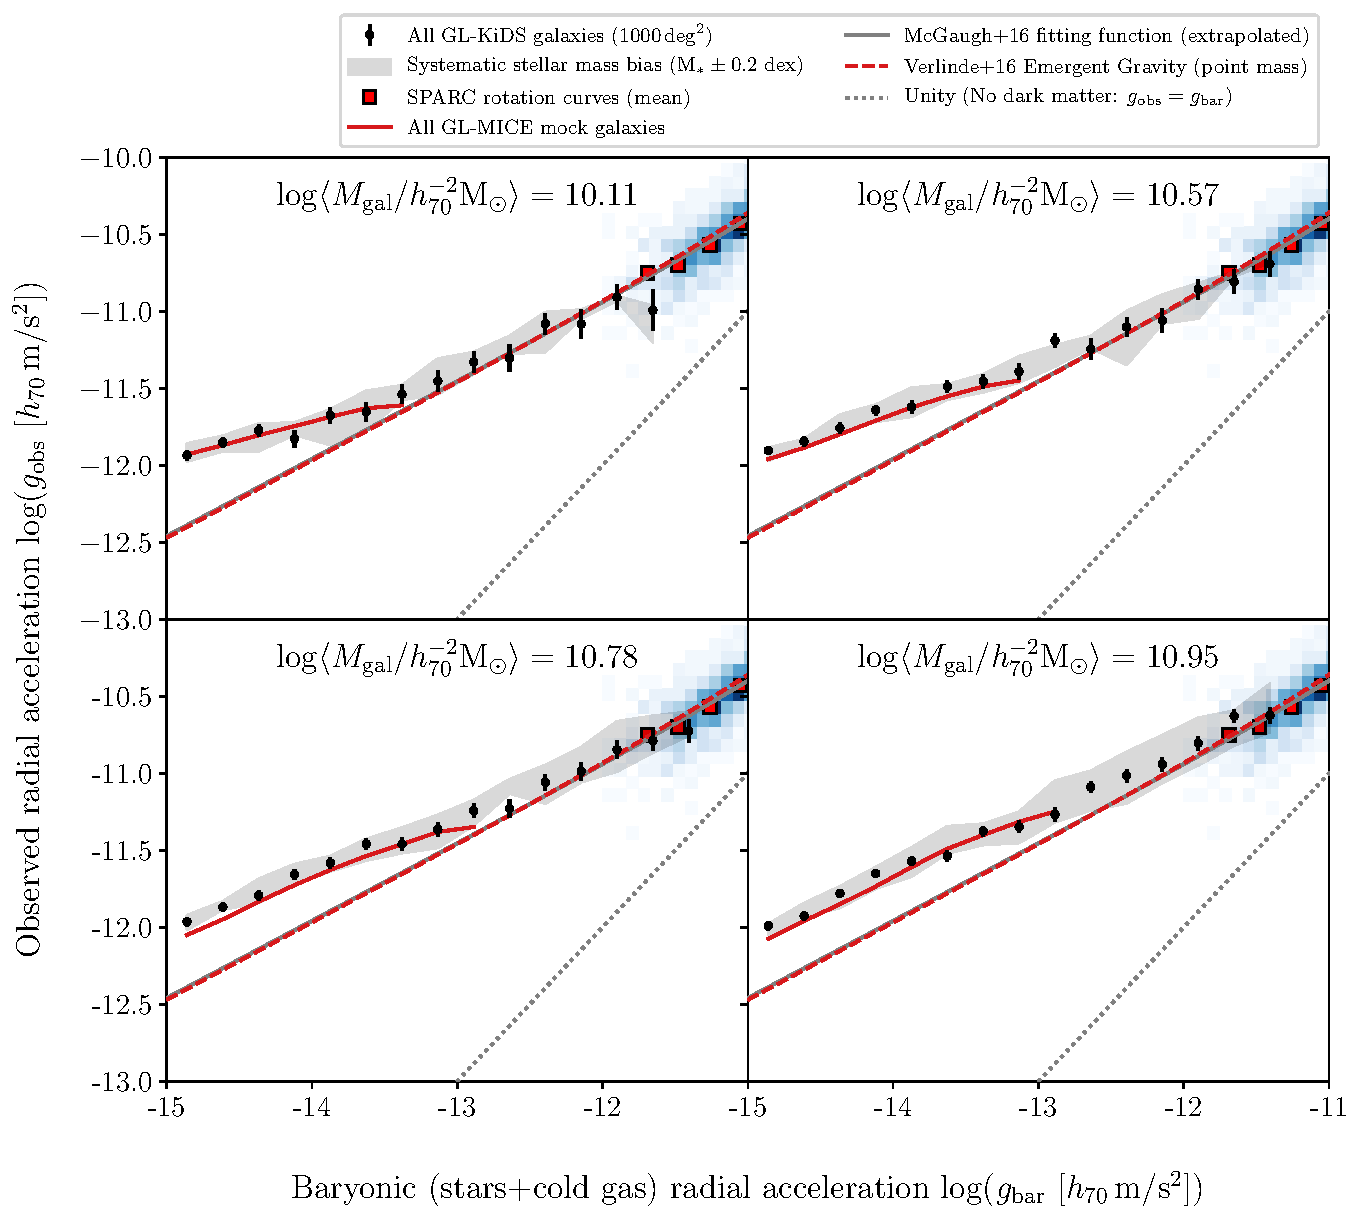
\includegraphics[width=\textwidth]{Figures/RAR_KiDS+MICE+Verlinde_4-massbins_all.pdf}
	\caption{The RAR measured for \emph{all} GL-KiDS lenses (black points with $1\sigma$ error bars) divided into 4 stellar mass bins, with the mean stellar mass of the lenses shown at the top of each panel. This figure primarily shows the effect on the RAR when the isolation criterion is not applied, which is quite significant and dependant on the stellar mass of the galaxies (which correlates with galaxy clustering). The extrapolated M16 and EG predictions (grey solid and red dashed lines) function merely as a reference, showing the approximate location of the isolated galaxy RAR. The predictions from the MICE simulation (red line) match with our observations, which shows that the clustering simulated within MICE, driving the low-acceleration upturn due to the `two-halo term', is indeed quite accurate.}
	\label{fig:RAR_kids_mice_mstarbins_all}
\end{figure*}
%\end{comment}

%Plot: KiDS + MICE (4 stellar mass bins, isolated)
\begin{figure*}
	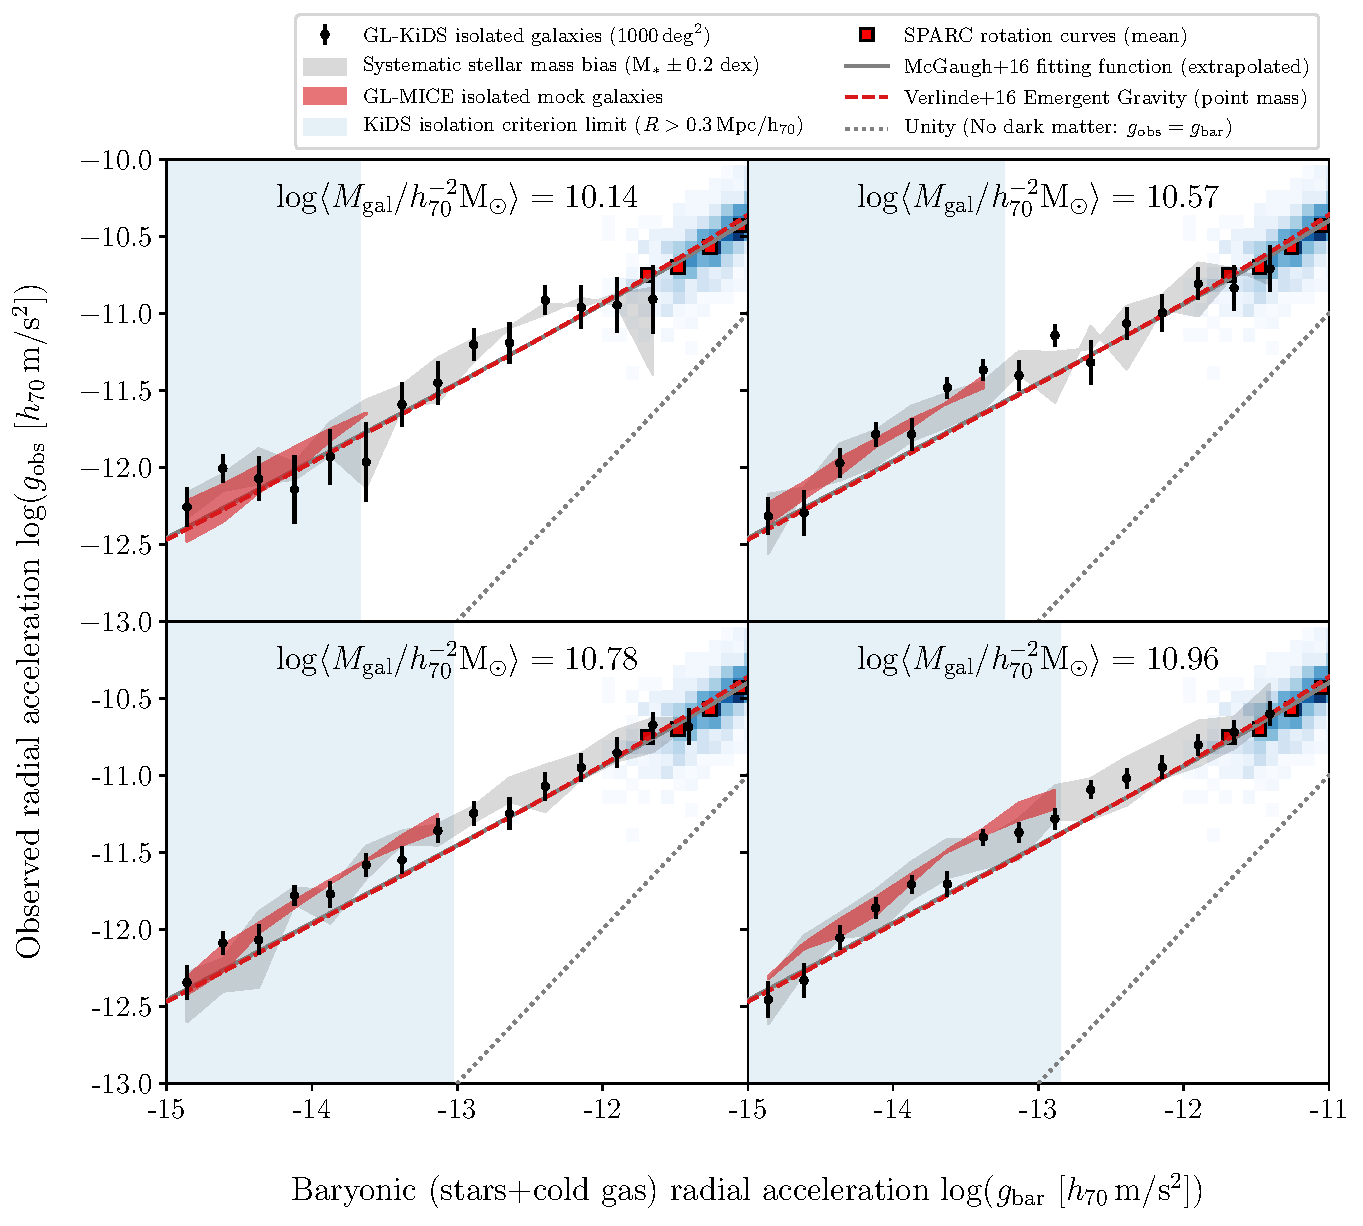
\includegraphics[width=\textwidth]{Figures/RAR_KiDS+MICE+Verlinde_4-massbins_isolated.pdf}
	\caption{The RAR measured for isolated GL-KiDS lenses (black points with $1\sigma$ error bars) divided into 4 stellar mass bins, with the mean stellar mass of the lenses shown at the top of each panel. At increasing stellar mass, the measurements seem to rise above the predictions from MOND (grey solid line) and EG (red dashed line). However, at scales larger than $R > 0.3 \hMpc$ (left of the blue dotted line) this could be caused by false positives in the isolated galaxy sample due to the GL-KiDS redshift uncertainty.}
	\label{fig:RAR_kids_mice_mstarbins}
\end{figure*}

%Plot: Dwarf galaxies (isolated)
\begin{figure*}
	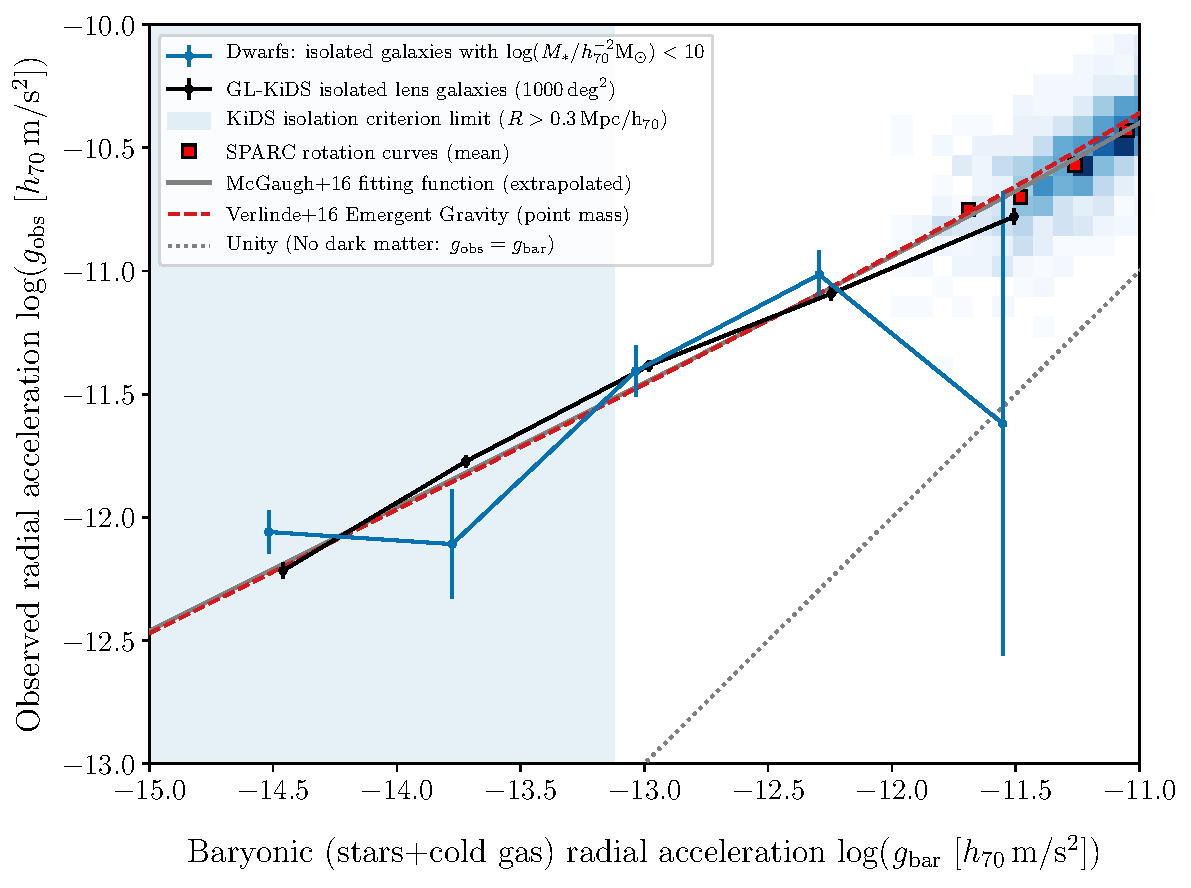
\includegraphics[width=0.8\textwidth]{Figures/RAR_KiDS+dwarfs_Nobins_isolated.pdf}
	\caption{The RAR measured for GL-KiDS lenses (points with $1\sigma$ error bars) for isolated `dwarfs' ($\log(M_\star/\hmsun)<10$, dark blue), compared to that of the full isolated galaxy sample ($\log(M_\star/\hmsun) < 11$, black). Due to the low $S/N$ ratio of the dwarf lensing signal, the number of $g\un{bar}$-bins is reduced from $15$ to $5$. We find that the RAR of dwarfs is consistent with that of our regular sample, and with the extrapolated M16 and EG predictions (grey solid and red dashed lines) which are shown as a reference.}
	\label{fig:RAR_kids_dwarfs}
\end{figure*}

We first split our GL-KiDS lenses into 4 samples based on their stellar mass $M_\star$. We select our $M_\star$-bins to obtain a similar $S/N$ ratio of the lensing signal in each bin, resulting in the following limits: $\log_{10}(M_\star/\hmsun) = [8.5,10.3,10.6,10.8,11.0]$. In Fig.~\ref{fig:RAR_kids_mice_mstarbins_all} we first show our GL-KiDS lensing measurements and MICE predictions for \emph{all} lens galaxies, without applying the isolation criterion. This is mainly meant to show the effect of selecting isolated galaxies on the RAR, which is quite striking. Again the MICE simulation is able to predict our measurements: $\chi\un{red}^2 = 57.18 / 33 = 1.73$ ($2.77 \sigma$). This shows that the clustering simulated within MICE, driving the low-acceleration upturn due to the `two-halo term', is indeed quite accurate, which can be expected since at $z<0.25$ it is constructed to reproduce the SDSS observations \cite[]{zehavi2011}.

But the main result is shown in Fig.~\ref{fig:RAR_kids_mice_mstarbins}, which shows the lensing measurements and predictions for \emph{isolated} galaxies split in 4 stellar mass bins. For each bin the mean stellar mass of the lenses, $\log_{10}\lan M_\star/\hmsun \ran = [10.14, 10.57, 10.78, 10.96]$, is shown at the top of the panel. At first glance, there appears to be an upward trend in the RAR of galaxies with larger $M_\star$, which moves the data away from the MOND and EG predictions. Indeed, quantifying the difference between the extended M16 fitting function and our measurement at \emph{all} scales would result in: $\chi\un{red}^2 = 127.49 / 60 = 2.12$, which (noting that the prediction for EG is very similar) would exclude both models at a $\sim5 \sigma$ level. However, at accelerations $g\un{bar}$ that correspond to scales larger than $R > 0.3 \hMpc$ (light blue area) an increasing signal is to be expected, since at these distances satellite galaxies missed by our isolation criterion might affect the measurement. Galaxies with higher stellar masses reside in denser neighbourhoods, and therefore tend to have more satellites \cite[see e.g.][]{baldry2006, bolzonella2010, brouwer2016}.

We therefore calculate the reduced $\chi^2$ values using only the data within $R < 0.3 \hMpc$. In this case the number of free parameters $N = 31$, and $\chi\un{red}^2 = 44.97 / 31 = 1.45$ for MOND and $46.63 / 31 = 1.50$ for EG respectively (corresponding to a standard deviation of $1.96$ and $2.10\sigma$). The remaining difference could again be alleviated by the possible stellar mass bias ($\Delta M_\star = 0.2 \dex$) which, if it shifts our results downward, would result in $\chi\un{red}^2 = 0.96$ for the extended M16 fitting function (with similar results for EG), in other words: a perfect fit. If shifted upwards, however, it would result in $\chi\un{red}^2=4.79$, a very bad fit. This again highlights the grave importance of accurate baryonic mass measurements in determining the RAR, in addition to deep lensing surveys that can detect satellites to down to very faint magnitudes \cite[such as the future Euclid survey;][]{laureijs2011}. As for the MICE simulation, it matches our measurements reasonably well in every $M_\star$ bin. As expected the result \emph{with} `offset' MICE redshifts during the isolated galaxy selection (which emulates effect of the GL-KiDS redshift uncertainty on the isolation criterion) performs better than without, resulting in an overall reduced $\chi^2$ value of $\chi\un{red}^2 = 54.02 / 30 = 1.80$ ($2.84 \sigma$).

As a final exploration of the different galaxy masses, we attempt to measure the RAR for the lightest lenses in GL-KiDS. Low-mass galaxies are of particular interest to DM/MG researchers as extreme examples that might show eccentric behaviour \citep{oman2016,dokkum2018,guo2020}, as well as those who attempt to extend the RAR to lower accelerations using galaxy rotation curves \citep{lelli2017b,paolo2019}. We therefore select a sample of `dwarfs': isolated galaxies with a stellar mass $M_\star<10^{10} \hmsun$ (whereas the full sample of isolated galaxies has $M_\star < 10^{11} \hmsun$, see Sect.~\ref{sec:isolation}). Since these galaxies are few, and have an even smaller effect on the path of light rays than heavier ones, we need to reduce the number of bins in $g\un{bar}$ from $15$ to $5$ to obtain sufficient $S/N$ radio in each bin. Fig.~\ref{fig:RAR_kids_dwarfs} shows the resulting RAR measurement of dwarfs compared to the full isolated sample (dark blue and black dots with $1\sigma$ error bars). We do not show the effect of a $0.2\dex$ systematic bias in $M\un{gal}$, because this would affect both results in the same way. We find that, within its large error bars, the RAR of the dwarfs is consistent with that of the full isolated sample; they both approximately follow the $g\un{obs}\propto\sqrt{g\un{bar}}$ relation expected by the extended M16 and EG predictions, which are shown as a reference (grey solid and red dashed lines). Hence, we do not find a significant difference in the RAR of dwarf galaxies.

\subsection{S\'ersic index and colour}
\label{sec:results-types}

% 2D histogram galaxy morphology
\begin{figure}
	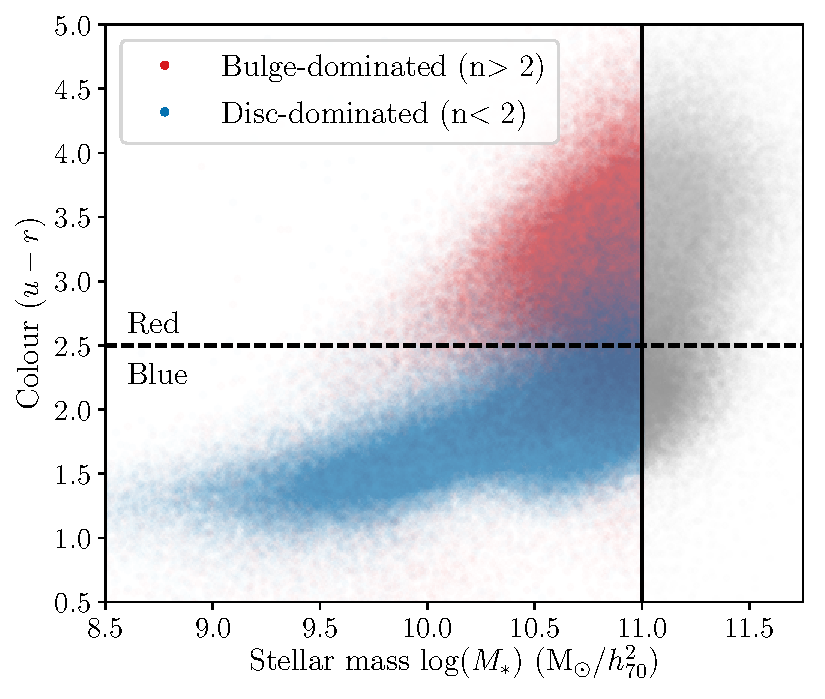
\includegraphics[width=\columnwidth]{Figures/galaxy_morphology_color_u-r.pdf}
	\caption{A 2D histogram of the $u-r$ colour and stellar mass of isolated GL-KiDS galaxies. We divide our galaxies into two types based on either S\'ersic index $n$ or $u-r$ magnitude. When dividing by S\'ersic index, we define bulge-dominated galaxies as those with $n>2$ and disc-dominated galaxies as those with $n<2$ (red and blue dots). When dividing colour we define red galaxies as those with $m\un{u} - m\un{r} > 2.5$ and blue galaxies as those with $m\un{u} - m\un{r} < 2.5$ (above and below the dashed horizontal line).}
	\label{fig:galtypes_scatterplot}
\end{figure}

% Red and blue mass histograms
\begin{figure}
	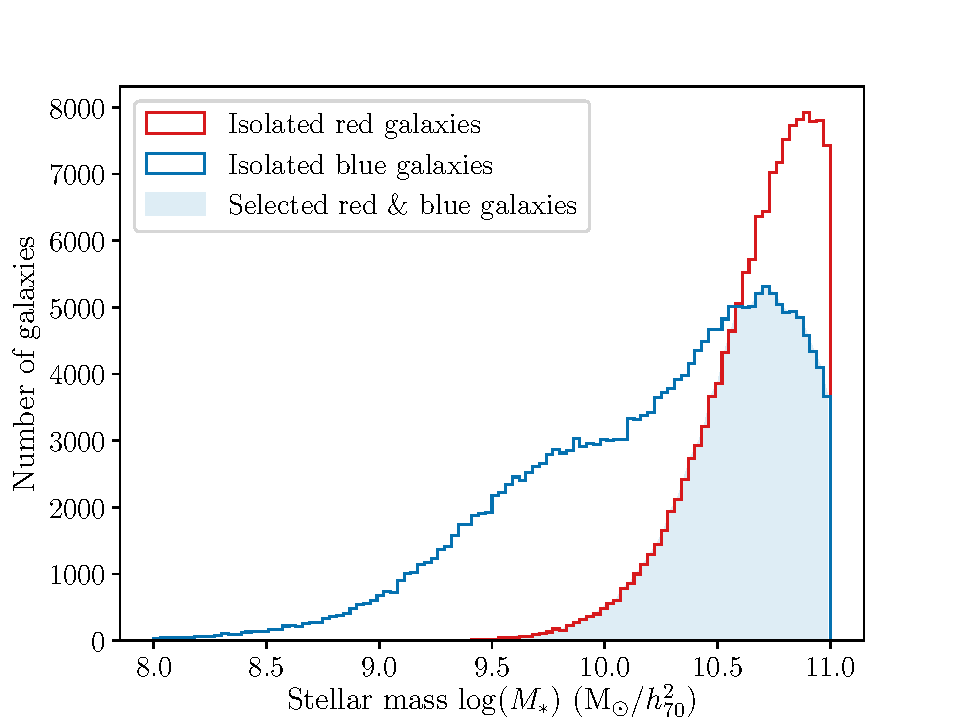
\includegraphics[width=\columnwidth]{Figures/mass_range_selection_offsetx0.pdf}
	\caption{The stellar mass histogram of the red and blue isolated GL-KiDS galaxies (red and blue lines), divided by $u-r$ colour ($m\un{u} - m\un{r} \lessgtr 2.5 \magn$). To isolate the effect of galaxy type on the RAR from that of $M_\star$, we aim to select two samples with the same stellar mass distribution. We therefore randomly remove galaxies from both samples until only the overlapping region (light blue area) remains.}
	\label{fig:galtypes_masshist}
\end{figure}


%Plot: KiDS (2 colour/S\'ersic bins, isolated)
\begin{figure*}
	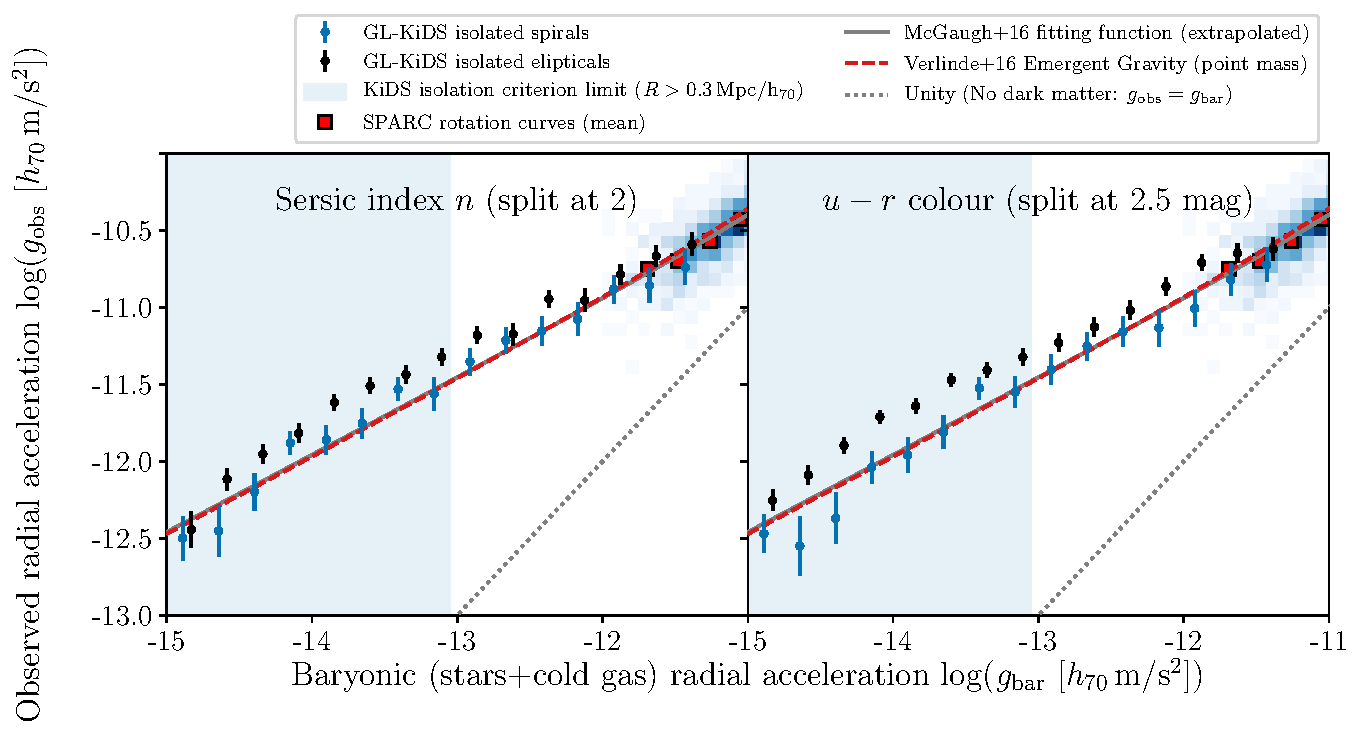
\includegraphics[width=\textwidth]{Figures/RAR_KiDS_galtypes_isolated_samemass.pdf}
	\caption{The RAR measured for isolated GL-KiDS lenses (points with $1\sigma$ error bars) divided into two galaxy types. In the left panel, the lenses are split by S\'ersic index ($n\gtrless2$) into bulge-dominated and disc-dominated galaxies, while in the right panel they are split by $u-r$ colour ($m\un{u} - m\un{r} \gtrless 2.5$) into red and blue galaxies. In both panels, we find a significant difference between the RAR measurements of the two galaxy types. The extrapolated M16 and EG predictions (grey solid and red dashed lines) are shown as a reference.}
	\label{fig:RAR_kids_galtypebins}
\end{figure*}

In the $\lcdm$ framework it is expected that the galaxy-to-halo-mass relation, and therefore the RAR, can be different for different galaxy types through their galaxy formation history \cite[]{dutton2010,matthee2017,posti2019,marasco2020}. This is in contrast with most MG models, which predict a fixed RAR (as is the case for MOND, and for EG at scales beyond the galaxy disc). Two parameters that correlate heavily with galaxy formation history are S\'ersic index and colour. We therefore measure the RAR for isolated galaxies split into two types based on either parameter: `bulge-dominated' and `disc-dominated' based on their S\'ersic index, and `red' and `blue' based on their $u-r$ colour.

The S\'ersic indices $n$ of all KiDS galaxies with $S/N > 50$ \citep[following][]{roy2018} are measured using the \textsc{2DPHOT} multi-purpose environment for 2D wide-field image analysis \cite[]{barbera2008}. For the colour split, we use the $u$ and $r$ magnitudes measured using the GAaP pipeline (see Sect.~\ref{sec:kids}). In Fig.~\ref{fig:galtypes_scatterplot} the $u-r$ colour versus stellar mass distribution of isolated galaxies shows our two selections: the split based on S\'ersic index defines bulge-dominated galaxies as those with $n > 2$ and disc-dominated galaxies as those with $n<2$ (red and blue points, respectively), whereas the split based on $u-r$ colour defines red galaxies as those with $m\un{u} - m\un{r} > 2.5 \magn$ and blue galaxies as those with $m\un{u} - m\un{r} < 2.5 \magn$ (above and below the dashed horizontal line, respectively).

In both cases, we aim to select two samples with the same stellar mass distribution, \textcolor{black}{in order to isolate the effect of galaxy type on the RAR from that of $M_\star$. Although in MG theories \emph{neither} should have any effect on the RAR, finding a significantly different RAR at equal $M_\star$ would make the observation even more constraining, and moreover would have interesting implications for galaxy formation models in the $\lcdm$ framework.} In Fig.~\ref{fig:galtypes_masshist} we show the $M_\star$ histogram of the two types (in this case based on galaxy colour). From both samples, we remove galaxies until only the overlapping section of both mass distributions remains. In the ideal case this should give us two samples (red and blue galaxies) with equal stellar mass distributions, shown by the light blue region.

However, the statistical uncertainty in the $M_\star$ measurements could cause a systematic shift in the two $M_\star$ distributions resulting from Eddington bias \cite[]{eddington1913}. We estimate the size of this bias by adding a random offset to the true $\log_{10}(M_\star)$ measurements of GL-KiDS before selecting the two `equal' stellar mass distributions for red and blue galaxies. Based on our estimate of the statistical uncertainty in the GL-KiDS $M_\star$ (see Sect.~\ref{sec:gamalike_kids}), we draw the random offsets from a lognormal distribution with $\sigma = 0.12 \dex$. When looking at the underlying true stellar mass distributions we find that they are indeed not equal, but that the mean stellar masses $\lan M\un{\star,r} \ran$ and $\lan M\un{\star,b} \ran$ of the red and blue samples differ by $0.026 \dex$. Of course, this method overlooks that fact that the measured $M_\star$ distribution already contains scatter, and is therefore not the \emph{true} $M_\star$ distribution. Indeed when we apply the random offset multiple times, we see the Eddington bias decreasing with $\sim7$~per~cent after every iteration. Therefore the true Eddington bias is likely to be slightly larger, around $0.028 \dex$.

Fig.~\ref{fig:RAR_kids_galtypebins} shows the lensing RAR of equal-mass GL-KiDS galaxies split by S\'ersic index (left panel) and $u-r$ colour (right panel). For this result, we focus on establishing whether there exists a significant difference between the RAR of the two types. Contrary to previous plots, the effect of a $0.2 \dex$ global systematic bias in $M_\star$ (normally shown by a grey band) is omitted, because this affects both measurements in the same way such that their relative difference does not change (the possibility of a colour- or S\'ersic index-dependent bias is discussed below).

We indeed observe a significant difference between the RAR measurements of the two galaxy types. To quantify this difference, we measure both the reduced $\chi^2$ and the mean ratio between the RAR measurements. The $\chi\un{red}^2$ equals $75.73 / 15 = 5.05$ for the lenses split by S\'ersic index, and $147.51 / 15 = 9.83$ for those split by $u-r$ colour. Taking the full covariance matrix into account we find that even the S\'ersic index split, which displays the smallest offset, results in RAR difference with a $6.25 \sigma$ significance. The mean ratio between the two RAR measurements $\log_{10}(\delta g\un{obs}^{\rm r/b}) = \log_{10}\left( \langle g\un{obs,r} / g\un{obs,b}\rangle \right)$ is $0.17 \dex$ and $0.26 \dex$ respectively. Here we have assumed that to first order, the uncertainty in the KiDS photo-z's affects the isolated galaxy selection of both galaxy types in the same way, allowing us to include the full acceleration range into our comparison. But even when we remove all data-points beyond the KiDS isolation criterion limit, we obtain a difference of $0.14$ and $0.19 \dex$ for the S\'ersic and colour split respectively, where the latter has a significance of $3.37 \sigma$.

However, these conclusions assume that the stellar mass estimates of the two populations are unbiased. To find whether our results are robust we estimate the systematic stellar mass bias between the two types, defined as: $\log_{10}(\delta M_\star^{\rm r/b}) = \log_{10}\left( \langle M_\star\rangle\un{r} / \langle M_\star\rangle\un{b} \right)$, that would be required to resolve the difference between their two RAR measurements. When trying to estimate the effect of this bias on the RAR, we have to take into account that $\delta M^{\rm r/b}_\star$ affects both the estimated acceleration from baryonic mass $g\un{bar}$ (directly) and the observed acceleration $g\un{obs}$ (indirectly, through the equal-mass selection). The bias in baryonic acceleration scales linearly with the bias in $M_\star$, such that: $\log_{10}(\delta g^{\rm r/b}\un{bar}) = \log_{10}(\delta M^{\rm r/b}_\star)$. Throughout this work, the observed relation between $g\un{bar}$ and $g\un{obs}$ at the scales measured by lensing has approximately followed $g\un{obs} \propto \sqrt{g\un{bar}}$. This means that we can roughly estimate the effect on $g\un{obs}$ as: $\log_{10}(\delta g^{\rm r/b}\un{obs}) \approx {\log_{10}(\delta M^{\rm r/b}_\star)} \, / \, {2}$. Since our measured difference $\delta g\un{obs} \gtrsim 0.2 \dex$, this means ${\log_{10}(\delta M^{\rm r/b}_\star)}$ should be  $\gtrsim 2 \log_{10}(\delta g^{\rm r/b}\un{obs}) = 0.4 \dex$. That is, our observed difference could be resolved should by a systematic stellar mass bias between the two types $\gtrsim 0.4 \dex$ (due to, e.g., Eddington bias, systematic variation of the IMF, SPS model inaccuracies, etc.).

As described above, we have estimated the effect of Eddington bias to be around $0.028 \dex$ in stellar mass. It is thus very unlikely that the difference we observe is caused exclusively by Eddington bias. In order to estimate the size of any other systematic biases, we compare GL-KiDS' $M\un{\star,ANN}$ with GAMA's $M\un{\star,G}$ of the same galaxies. After selecting our samples of blue and red galaxies with the same $M\un{\star,ANN}$ distribution as described above, we indeed find that the $M\un{\star,G}$ distributions are not exactly equal: $\langle M_\star \rangle\un{r} / \langle M_\star\rangle\un{b} = 1.37$, corresponding to $0.14 \dex$. This indicates that using different sets of observations and models to measure $M_\star$ can cause a systematic bias between red and blue galaxies, but that this effect is too small to reach the $\gtrsim 0.4 \dex$ difference in $M_\star$ needed to explain the $\gtrsim 0.2 \dex$ difference in the measured RAR. Even when combined, the Eddington plus overall systematic measurement bias is at most $0.17 \dex$, not even half of what is needed. Note that this bias estimation has been done using the types split by $u-r$ colour; when split by S\'ersic index, the Eddington and other systematic biases between bulge- and disc-dominated galaxies are even smaller ($0.021$ and $0.12 \dex$ respectively).

If confirmed, the found difference in the RAR based on galaxy type might prove difficult to explain within MG frameworks. In a $\lcdm$ context, it would point to a difference in the SHMR for different galaxy types. Indeed, another recent KiDS-1000 lensing study by \cite{taylor2020} found that, within a narrow stellar mass range near the knee of the SHMR ($M_\star \sim 2-5\E{10} \hmsun$), galaxy halo mass varied with galaxy colour, star formation rate, effective radius and Sérsic index. Their observations showed that canonically `early type' (red, bulge dominated) galaxies had larger halo masses than `late type' (blue, disc-dominated) galaxies. Even more recently, \cite{correa2020} used SDSS data with morphological classifications from Galaxy Zoo to find that, at fixed halo mass (in the range $10^{11.7} - 10^{12.9} \msun$), the median stellar mass of SDSS disc galaxies was a factor $1.4$ higher than that of ellipticals. They found this to be in agreement with simulations from EAGLE, where haloes hosting disc galaxies are assembled earlier than those hosting ellipticals, therefore having more time for gas accretion and star formation. The higher values of $g\un{obs}$ for red/bulge-dominated galaxies that we find in Fig. \ref{fig:RAR_kids_galtypebins} of this work, are in agreement with the results of both these studies.


\section{Discussion and conclusion}
\label{sec:discon}

Using galaxy-galaxy lensing (GGL) with $1000 \deg^2$ of Kilo Degree Survey data (KiDS-1000) we have extended the radial acceleration relation of isolated galaxies by nearly $2$ orders of magnitude in gravitational acceleration $g\un{obs}$, compared to previous measurements based on rotation curves \cite[most notably][M16]{mcgaugh2016}. To compute the lensing RAR, we converted our excess surface density profiles $\Delta\Sigma(R)$ into the observed gravitational acceleration $g\un{obs}$, and our galaxy masses (measured using 9-band KiDS+VIKING photometry) into $g\un{bar}$. These measurements allowed us to perform unprecedented tests of two modified gravity models: MOND and Emergent Gravity, as well as tests of $\lcdm$ in the form of the N17 analytical model, and the MICE (N-body + semi-analytic) and BAHAMAS (hydrodynamical) simulations. Our conclusions from these observational tests are as follows:

\begin{itemize}

	\item Fig.~\ref{fig:Vrot_kids_verlinde_mice}: We find that `rotation curves' of isolated galaxies measured through GGL remain approximately flat at scales far beyond the visible disc ($0.03 < R < 3 \hMpc$). At the accelerations corresponding the outskirts of observable galaxies ($R \approx 30\hkpc$), our lensing results are in excellent agreement with the SPARC rotation curves \cite[]{lelli2016b}. It is very reassuring that these two measurements, obtained by two very different methods, exactly match at the scales where their domains (respectively within and outside of the observable galaxy) overlap.
	
	\item Fig.~\ref{fig:RAR_kids_gama_verlinde}: At the low accelerations corresponding to GGL scales, the lensing RAR of isolated galaxies approximately follows a $g\un{obs} \propto \sqrt{g\un{bar}}$ relation. This is in agreement with the expectations from EG (Eq. \ref{eq:rar_verlinde}) and MOND (which we take to be the M16 fitting function, Eq. \ref{eq:rar_mcgaugh}, extrapolated to larger scales). At low accelerations both these models predict a direct relation between observed and baryonic acceleration of this form, with a very similar proportionality constant\footnote{The proportionality constant $c H_0 / 6$ in EG is almost equal to the value of $g\un{\dagger}$ found by M16, which is again equal to the $a_0=1.2\E{-10} \mpss$ canonical in MOND.} of $\sim1.2\E{-10} \, \mpss$. This reinforces the results of \cite{brouwer2017}, who found that EG provides a good description of ESD profiles measured using $180 \deg^2$ of KiDS-GAMA data, but with a 5 times larger survey area.
	
	\item Fig.~\ref{fig:RAR_kids_gama_Navarro}: When converted into an (apparent) mass distribution using Newton's law of gravity (Eq. \ref{eq:grav}) the relation $g\un{obs} \propto \sqrt{g\un{bar}}$ corresponds to a SIS density profile: $\rho \propto r^{-2}$ (Eq. \ref{eq:rho_SIS}). The N17 analytical model is based on isolated galaxies with DM haloes following an NFW density profile, which has an $r^{-3}$ radial dependence beyond the scale radius. So although the N17 model performs well at the smaller scales of M16 rotation curves, at the larger scales probed by lensing we found that its prediction bends down with respect to our measurement. We concluded that a simple analytical $\lcdm$ model is not sufficient to describe our observations, and that a fair comparison requires numerical simulations such as BAHAMAS and MICE, which can mimic the measurement more faithfully.
	
	\item Fig.~\ref{fig:RAR_kids_mice_bahamas}: We found that the BAHAMAS simulation underestimates our GL-KiDS lensing RAR. This is caused by a bias in the SHMR of isolated galaxies in these simulations for which there is currently no strong observational evidence: they have stellar masses typically $3$ times higher at fixed halo mass than their non-isolated counterparts. Interestingly, the BAHAMAS RAR still has approximately the correct low-acceleration slope, rather than a steeper slope as would naively be predicted based on the $\rho\propto r^{-3}$ outer slopes of the simulated DM haloes. The prediction from MICE (only feasible at low accelerations due to the limited resolution of the simulated lensing measurements) matches our RAR measurements very well, again in contrast with the expectation for DM haloes with NFW density profiles. The additional lensing power at large radii might be caused by large scale structure along the line-of-sight (LOS) to the source, in spite of our efforts to select isolated galaxies. This highlights the crucial importance of simulating the entire measurement process (where possible) when making theoretical predictions.
	
	\item Fig.~\ref{fig:RAR_kids_mice_mstarbins}: When we measured the lensing RAR for galaxy samples split by stellar mass $M_\star$, there appeared to be a small upward trend away from the fixed predictions of MOND and EG. However, at scales beyond the KiDS isolation criterion limit ($R>0.3 \hMpc$), this could be caused by satellite or companion galaxies missed by the isolated galaxy selection due to the GL-KiDS redshift uncertainty. Also, as with all previous results, the shift in the RAR caused by a $0.2 \dex$ systematic bias in $M_\star$ (which is the current state-of-the-art limit) can make the difference between a perfect fit and a significant exclusion of the MG models. This highlights the crucial importance of accurate baryonic mass measurements in determining the RAR, in addition to deep lensing surveys that can detect satellites to down to very faint magnitudes \cite[such as the future Euclid survey;][]{laureijs2011}. The MICE prediction, which is corrected for the GL-KiDS redshift uncertainty, again matches well to our data.
	
	\item Fig.~\ref{fig:RAR_kids_dwarfs}: We found no significantly different RAR, relative to the entire isolated lens sample, for a subsample of the lightest GL-KiDS lenses: isolated $M_\star < 10^{10} \hmsun$ `dwarf' galaxies.
	
	\item Fig.~\ref{fig:RAR_kids_galtypebins}: When we split galaxies into two types based on S\'ersic index or $u-r$ colour, we found at least a factor $1.5$ ($\simeq0.2 \dex$) difference between the respective lensing RAR measurements with a significance of at least $6.25 \sigma$. This observed difference could be resolved by a $\gtrsim 0.4 \dex$ systematic bias between the stellar masses of the two types. However, we calculated that the expected $M_\star$ bias (due to Eddington bias or systematic biases in the $M_\star$ measurement) is at most $0.17 \dex$. This variation in the RAR based on galaxy type, which is in agreement with \cite{taylor2020} and \cite{correa2020}, could be difficult to explain for MG models that predict a fixed relation between baryonic mass and the total gravitational potential.
	
	\item Throughout this work, we found that the field of GGL has reached a level of accuracy in the measurement of $g\un{obs}$ greater than that of the baryonic acceleration $g\un{bar}$. The fact that we have no accurate measurements of hot gas at large radii, and the ambiguity around the cosmological `missing baryons', forces us to limit $g\un{bar}$ to the contributions of stars and cold gas. In addition, the current $0.2 \dex$ systematic uncertainty in $M_\star$ prevents us from definitively excluding any of the models we test. This shows that, if we want to have any hope of testing DM and MG models using the next generation of cosmological lensing surveys (such as Euclid and LSST), we also need to focus on the models and observations needed to accurately measure the baryonic mass distribution in and around galaxies.
\end{itemize}

It is quite amazing that the extrapolated M16 fitting function (Eq. \ref{eq:rar_mcgaugh}), which approximately corresponds to the prediction of both MG models (EG and MOND), holds to scales of $3 \hMpc$ for isolated galaxies. However, a fundamental limitation of this measurement remains that the diffuse gas surrounding galaxies remain difficult to measure, and have therefore not been included in this observational study. More baryonic mass at large scales would increase the value of $g\un{bar}$, causing a steeper downwards slope in our RAR measurement (for an example, see the lower panel of Fig.~\ref{fig:missing-baryons}). A convincing detection of these components would move the observed RAR away from the MG predictions (which are fixed at $g\un{bar} \propto \sqrt{g\un{obs}}$) and towards the DM predictions (where $g\un{bar}$ and $g\un{obs}$ are independent), whereas a robust non-detection would strengthen the position of MG models. In any case, the fact that galaxy `rotation curves' appear to continue approximately flat out to $R=3\hMpc$ (where observations are bound to encounter surrounding galaxies) is difficult to explain in a $\lcdm$ framework that predicts `NFW-like' haloes. However, our analysis of the MICE simulations shows that the combination of the lenses and the additional structure along the LOS can yield an ESD profile consistent with an $\sim r^{-2}$ density profile for isolated galaxies, even though the lenses have an intrinsic $\sim r^{-3}$ outer profile.

We find that the lensing RAR is a promising method to be used by future cosmological surveys to distinguish between MG and DM models. This can be done by measuring the RAR including large-scale baryonic mass observations as described above; by simply performing the same comparison with even more accurate lensing and stellar mass measurements; or by further exploring our found `shift' in the RARs of different galaxy types. All these options require that systematic biases in the stellar and other baryonic mass measurements be reduced.


\section*{Acknowledgements}
\textcolor{red}{To be adjusted according to co-authors.}

%\begin{comment}
We are indebted to Ian McCarthy, who provided the BAHAMAS data products used in our analysis.

KAO acknowledges support by the Netherlands Foundation for Scientific Research (NWO) through VICI grant 016.130.338 to M. Verheijen, and support from the European Research Council (ERC) through Advanced Investigator grant to C.S. Frenk, DMIDAS (GA 7786910).

We are grateful to \url{https://math.stackexchange.com} user Paul Enta for providing an expression for one of the integrals needed in Appendix~\ref{sec:appendix_invert_esd}.

This work is partly based on tools and data products produced by GAZPAR operated by CeSAM-LAM and IAP.

% M. Bilicki is supported by the Netherlands Organization for Scientific Research, NWO, through grant number 614.001.451. C. Heymans acknowledges support from the European Research Council under grant number 647112. H. Hoekstra acknowledges support from Vici grant 639.043.512, financed by the Netherlands Organization for Scientific Research. K. Kuijken acknowledges support by the Alexander von Humboldt Foundation. H. Hildebrandt is supported by an Emmy Noether grant (No. Hi 1495/2-1) of the Deutsche Forschungsgemeinschaft. P. Schneider is supported by the Deutsche Forschungsgemeinschaft in the framework of the TR33 `The Dark Universe'. E. van Uitert acknowledges support from an STFC Ernest Rutherford Research Grant, grant reference ST/L00285X/1.

Computations for the $N$-body simulations were performed in part on the Orcinus supercomputer at the WestGrid HPC consortium (\url{www.westgrid.ca}), in part on the GPC supercomputer at the SciNet HPC Consortium. SciNet is funded by: the Canada Foundation for Innovation under the auspices of Compute Canada; the Government of Ontario; Ontario Research Fund - Research Excellence; and the University of Toronto.

This research is based on data products from observations made with ESO Telescopes at the La Silla Paranal Observatory under programme IDs 177.A-3016, 177.A-3017 and 177.A-3018, and on data products produced by Target OmegaCEN, INAF-OACN, INAF-OAPD and the KiDS production team, on behalf of the KiDS consortium. OmegaCEN and the KiDS production team acknowledge support by NOVA and NWO-M grants. Members of INAF-OAPD and INAF-OACN also acknowledge the support from the Department of Physics \& Astronomy of the University of Padova, and of the Department of Physics of Univ. Federico II (Naples).

GAMA is a joint European-Australasian project based around a spectroscopic campaign using the Anglo-Australian Telescope. The GAMA input catalogue is based on data taken from the Sloan Digital Sky Survey and the UKIRT Infrared Deep Sky Survey. Complementary imaging of the GAMA regions is being obtained by a number of independent survey programs including GALEX MIS, VST KiDS, VISTA VIKING, WISE, Herschel-ATLAS, GMRT and ASKAP providing UV to radio coverage. GAMA is funded by the STFC (UK), the ARC (Australia), the AAO, and the participating institutions. The GAMA website is \url{www.gama-survey.org}.

This work has made use of CosmoHub \cite[]{carretero2017,tallada2020}. CosmoHub has been developed by the Port d'Informaci{\'o}n Cient{\'i}fica (PIC), maintained through a collaboration of the Institut de F{\'i}sica d'Altes Energies (IFAE) and the Centro de Investigaciones Energ{\'e}ticas, Medioambientales y Tecnol{\'o}gicas (CIEMAT), and was partially funded by the ``Plan Estatal de Investigaci{\'o}n Cient{\'i}fica y T{\'e}cnica y de Innovaci{\'o}n'' program of the Spanish government.

This work has made use of {\scshape python} (\url{www.python.org}), including the packages {\scshape numpy} (\url{www.numpy.org}) and {\scshape scipy} (\url{www.scipy.org}). Plots have been produced with {\scshape matplotlib} \cite[]{hunter2007}. The mock shear profiles from MICE are computed using {\scshape TreeCorr} (\url{https://pypi.python.org/pypi/TreeCorr}).

\emph{Author contributions:} All authors contributed to the development and writing of this paper. The authorship list is given in three groups: the lead authors (M. Brouwer, K. Oman), followed by two alphabetical groups. The first alphabetical group includes those who are key contributors to both the scientific analysis and the data products. The second group covers those who have either made a significant contribution to the data products, or to the scientific analysis.

%\end{comment}
%%%%%%%%%%%%%%%%%%%%%%%%%%%%%%%%%%%%%%%%%%%%%%%%%%

%%%%%%%%%%%%%%%%%%%% REFERENCES %%%%%%%%%%%%%%%%%%

% The best way to enter references is to use BibTeX:

\bibliographystyle{mnras}
\bibliography{biblio}


%%%%%%%%%%%%%%%%%%%%%%%%%%%%%%%%%%%%%%%%%%%%%%%%%%

%%%%%%%%%%%%%%%%%%%%%%%%%%%%%%%%%%%%%%%%%%%%%%%%%%

\appendix
\onecolumn
\section{Excess surface density profile of a piece-wise power law volume density profile}
\label{sec:appendix_invert_esd}

\noindent The excess surface density profile is measured in a series of discrete radial bins with edges $R_m$. The representative value at the centre of the bin -- here we define the bin centre as $\frac{1}{2}(R_m+R_{m+1})$, i.e. not the `logarithmic centre' $\sqrt{R_mR_{m+1}}$, which ensures accuracy in the calculation of the mean enclosed surface density -- is $\Delta\Sigma_m=\overline{\Sigma}_m-\Sigma_m$, where $\overline{\Sigma}_m$ is the mean surface density within $\frac{1}{2}(R_m+R_{m+1})$ and $\Sigma_m$ is the surface density averaged over the interval $[R_m,R_{m+1})$. We give an expression for this discrete excess surface density profile in terms of the parametric form for $\rho(r)$ given in Eq.~\ref{eq:rho_piecewise_powerlaw}.

The mean enclosed surface density is:

\begin{align}
\overline{\Sigma}_m &= \frac{1}{\pi R_mR_{m+1}}\left[I_1(0, \sqrt{R_0R_1}, \tilde{a}_0, \tilde{b}_0) + 
\sum_{k=0}^m I_1(\sqrt{R_mR_{m+1}},\sqrt{R_{m+1}R_{m+2}}, \tilde{a}_m, \tilde{b}_m)\right]\\
  \tilde{a}_m &= \frac{\ln(\Sigma_{m+1})-\ln(\Sigma_m)}{\frac{1}{2}\left(\ln(R_{m+2})-\ln(R_m)\right)}\\
  \tilde{b}_m &= \ln(\Sigma_m) - \frac{1}{2}\tilde{a}_m\ln(R_mR_{m+1})\\
  I_1(R_i,R_j,\tilde{a},\tilde{b}) &= \frac{2\pi e^{\tilde{b}}}{\tilde{a}+2}\left(R_j^{a+2} - R_i^{a+2}\right)
\end{align}
\noindent and the local surface density is given by:
\begin{align}
  \Sigma_m &= \sum_{n=0}^{N-1}
  \begin{cases}
    0 & {\rm if}\ r_{n+1} < R_m\\
    \frac{4e^{b_n}}{R_{m+1}^2-R_m^2} \left(-I_2(r_{n+1},R_m,a_n)\right) & {\rm if}\ r_n < R_m\ {\rm and}\ R_m \leq r_{n+1} < R_{m+1}\\
    \frac{4e^{b_n}}{R_{m+1}^2-R_m^2} \left(I_2(r_{n+1},R_{m+1},a_n)-I_2(r_{n+1},R_m,a_n)\right) & {\rm if}\ r_n < R_m\ {\rm and}\ r_{n+1} \geq R_{m+1}\\
    \frac{4e^{b_n}}{R_{m+1}^2-R_m^2} (I_2(r_{n+1},r_n,a_n)-I_2(r_{n+1},R_m,a_n)\\ \quad +I_2(r_n,R_m,a_n)+I_2(r_{n+1},R_{m+1},a_n)\\ \quad -I_2(r_{n+1},r_n,a_n)) & {\rm if}\ R_m \leq r_n < R_{m+1}\ {\rm and}\ r_n \geq R_{m+1}\\
    \frac{4e^{b_n}}{R_{m+1}^2-R_m^2} (I_2(r_{n+1},R_{m+1},a_n)-I_2(r_{n+1},R_m,a_n)\\ \quad -I_2(r_n,R_{m+1},a_n)+I_2(r_n,R_m,a_n)) & {\rm if}\ r_n \geq R_{m+1}\\
    \frac{4e^{b_n}}{R_{m+1}^2-R_m^2} (I_2(r_{n+1},r_n,a_n)-I_2(r_{n+1},R_m,a_n)\\ \quad +I_2(r_n,R_m,a_n)-I_2(r_{n+1},r_n,a_n)) & {\rm if}\ r_n \geq R_m\ {\rm and}\ r_{n+1} < R_m\\
  \end{cases}\\
  I_2(r,R,a) &=
  \begin{cases}
    -\frac{1}{3}R^{a+3}\left(\frac{r^2}{R^2}-1\right)^{\frac{3}{2}}{}_2{\rm F}_1\left(\frac{3}{2},-\frac{a}{2};\frac{5}{2};1-\frac{r^2}{R^2}\right) & {\rm if}\ r\ {\rm is}\ {\rm finite}\\
    \frac{\sqrt{\pi}}{2}\frac{\Gamma\left(-\frac{a+1}{2}\right)}{\Gamma\left(-\frac{a}{2}\right)}\frac{R^{a+3}}{a+3} & {\rm if}\ r=\infty
  \end{cases}
\end{align}
where ${}_2{\rm F}_1(\cdot,\cdot;\cdot;\cdot)$ is the Gaussian hypergeometric function and $\Gamma(\cdot)$ is the Gamma function. We assume that the power law slope in the innermost bin continues to $r=0$, and that that in the outermost bin continues to $r\rightarrow\infty$. When inverting $\Delta\Sigma(\rho)$, we impose uninformative priors on the power law slopes except those constraints required to guarantee that the total mass is finite and the calculation is numerically stable.

% Don't change these lines
\bsp	% typesetting comment
\label{lastpage}
\end{document}

% End of mnras_template.tex
